\documentclass[11pt]{article}
\usepackage[a4paper,margin=1in]{geometry}
\usepackage{amsmath,amssymb,amsthm,mathtools}
\usepackage{booktabs}
\usepackage{textcomp}
\usepackage[T1]{fontenc}
\usepackage{lmodern}
\usepackage{microtype}
\usepackage{graphicx}
\usepackage{caption}
\captionsetup{font=small,labelfont=bf}
\usepackage[numbers,sort&compress]{natbib}
\usepackage[hidelinks]{hyperref}
\graphicspath{{figures/}}

\newtheorem{theorem}{Theorem}
\newtheorem{proposition}{Proposition}
\newtheorem{lemma}{Lemma}
\newtheorem{corollary}{Corollary}
\theoremstyle{definition}
\newtheorem{definition}{Definition}
\theoremstyle{remark}
\newtheorem{remark}{Remark}

\newcommand{\E}{\mathbb{E}}
\newcommand{\Prob}{\mathbb{P}}
\newcommand{\F}{\mathcal{F}}
\newcommand{\Sphere}{\mathcal{S}}
\newcommand{\Aspace}{\mathcal{A}}
\newcommand{\Wmap}{\mathsf{W}}
\newcommand{\sfas}{\textsc{sfas}}
\newcommand{\TV}{\operatorname{TV}}

\title{\bfseries \textsc{someopark-football-agentic-simulator}:\\
A Multi-Agent LLM System for Football Simulation with\\
Low-Rank Team Identity and Stabilised Emergent Possession}

\author{Lingxiao Xu\thanks{Correspondence: \texttt{admin@someopark.com}. The system described here was designed and implemented in full by the author; code and the match corpus reproduce every figure and number.}\\
\normalsize Someo Park\\
\normalsize \texttt{admin@someopark.com}}

\date{\today}

\begin{document}
\maketitle

\begin{abstract}
\noindent We present \textsc{someopark-football-agentic-simulator} (\sfas), a multi-agent system in which twenty-two large-language-model (LLM) agents play a full ninety-minute football match. The design is deliberately minimal: every frame, the system broadcasts one shared, coarsened \emph{world map} to all agents; each agent, queried in parallel and in isolation, returns an intent or a ball action; and a single deterministic \emph{resolution operator} advances the physical state. The agents never exchange messages. Team identity is not a prompt but a \emph{parameter} --- each of forty-eight national teams is a rank-$16$ low-rank adapter over one shared base policy, distilled from player attributes and statistical tendencies and hot-swapped at serve time --- and pre-match tactics are grounded in a knowledge graph that supplies a handful of control set-points. This paper is a \emph{systems} contribution: we describe the architecture, the per-team adaptation pipeline, and the knowledge-graph grounding, and we explain \emph{why the system is stable}. Two emergent failure modes that sink the naive design --- possession ``snowballing'' to a monopoly, and formations collapsing onto the ball --- are shown to be generic dynamical phenomena, each cured by a control law with a sharp, closed-form threshold: a recent-share feedback that removes a pitchfork bifurcation once its gain exceeds $g^\star=4(\beta-1)$, and a convex intent-anchoring blend that guarantees a strictly positive lower bound $(1-\lambda)^2S^2$ on formation spread. We validate the system on a $75$-match corpus over seven simulated 2026 World-Cup fixtures spanning the strength spectrum, from evenly matched pairs to heavy mismatches: the standard match statistics land in independent realism bands (pass completion in-band in all $150$ team-matches); a six-match open-loop ablation reproduces the predicted bimodal possession monopoly; play is competitive rather than scripted --- in the five one-sided fixtures the out-matched side still wins $11\%$ of matches, e.g.\ Paraguay beating France $1$--$0$ while conceding $69.5\%$ possession --- and the dominant side's possession is venue-symmetric ($68.2\%$ at home vs $68.6\%$ away across the two most mismatched fixtures), never a monopoly. The result is a small, reproducible blueprint for many-agent LLM simulations in which coordination is a property of a shared environment rather than of communication, and in which emergent invariants are governed by identified control laws: the thresholds are analytic, and only the per-fixture operating points are learned, inside the stability region those thresholds guarantee.

\smallskip
\noindent\textbf{Keywords:} multi-agent systems; LLM agents; agentic simulation; emergent coordination; low-rank adaptation; knowledge graphs; decentralised control; sports simulation.
\end{abstract}

\section{Introduction}\label{sec:intro}

Large language models are increasingly deployed as \emph{agents}: they perceive a situation, decide, and act, in a loop \citep{park2023,wang2023survey,yao2023}. Most work studies one agent, or a handful of agents that \emph{talk} to each other \citep{li2023camel}. We are interested in the regime of \emph{many} LLM agents sharing one fast, adversarial, physically grounded world, and in the questions that regime raises but the single-agent literature does not answer: \textbf{(i)} how do agents that cannot communicate nonetheless coordinate into coherent collective behaviour, and \textbf{(ii)} when the collective behaviour is an emergent, self-reinforcing quantity, what keeps it realistic instead of letting it run away to a degenerate state?

We study these questions in the most demanding everyday instance of the regime --- a football match --- and build a system, \textsc{someopark-football-agentic-simulator} (\sfas), to answer them. A match is a closed twenty-two-agent system with a hard physical substrate (the ball is indivisible and conserved), rich individual heterogeneity, team identity, and a wealth of \emph{measurable} aggregate invariants --- possession share, pass-completion rate, shots, expected goals --- against which any simulator can be falsified. Unlike reinforcement-learning football environments, which train low-level motor policies from reward \citep{kurach2020,kitano1997}, \sfas{} treats each player as a \emph{language-model agent} that reasons over a symbolic view of the pitch and emits high-level intent; the appeal is interpretability and zero-shot tactical control (a team's style is a trained adapter and a knowledge-graph brief, not a reward schedule), and the challenge is that nothing in the LLM stack guarantees the emergent match will be realistic. Making it realistic, and understanding \emph{why} the fix works, is the content of this paper.

\paragraph{The system in one paragraph (Fig.~\ref{fig:arch}).} At each frame \sfas{} broadcasts a single \emph{world map} $w_t$ --- a coarsened, common description of all twenty-two positions (on a $6\times9$ zone grid), the ball, the score and the phase --- to every agent. Off the ball, each agent returns an \emph{intent} (a target zone and a posture); on the ball, the holder returns a categorical ball action (pass, shoot, cross, clear). Every agent acts on every frame: agents are queried in parallel and in isolation, simultaneously, with \emph{no} message channel between them and no turn order. A deterministic \emph{resolution operator} --- the physics substrate --- then takes the state and the twenty-two actions and produces the next state, resolving movement, passes, tackles, shots, offside and goals. Team identity is a rank-$16$ low-rank adapter over one shared base policy; pre-match tactical set-points come from a knowledge graph; and an outer calibration gate checks eleven aggregate statistics against real-football bands. The loop, run for $\approx4000$ frames, produces a complete match with a trajectory, a score and a full statistical line.

\begin{figure}[t]\centering
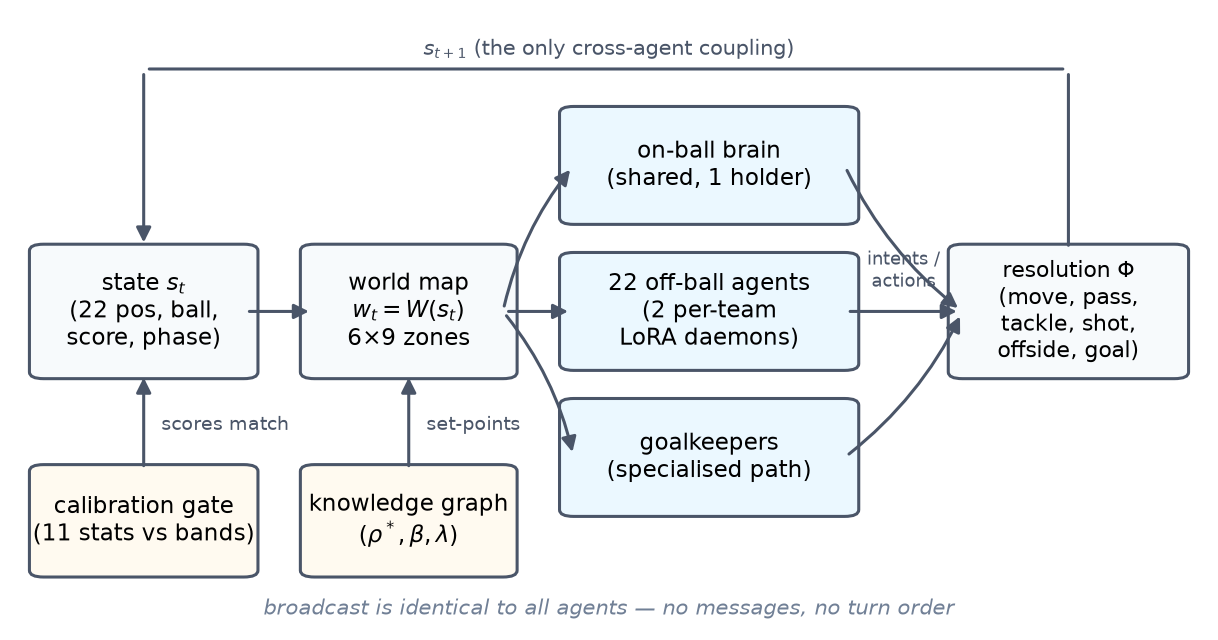
\includegraphics[width=0.96\textwidth]{fig_architecture.png}
\caption{The \sfas{} agentic loop. A shared world map is broadcast to twenty-two isolated agents (one shared on-ball ``brain'' policy and two per-team off-ball policies, each a LoRA over the shared base); their intents are merged only by the deterministic resolution operator $\Phi$, which advances the state. A knowledge graph supplies tactical set-points; a calibration gate scores the realised match. The recursion through $\Phi$ is the \emph{only} cross-agent coupling.}
\label{fig:arch}
\end{figure}

\paragraph{Why a naive build fails.} Assembled directly, the loop fails in two characteristic ways, and both are \emph{dynamical}, not implementational. First, possession \emph{snowballs}: a team that wins the ball early keeps it for the rest of the match (final shares of $80$--$90\%$), because holding the ball is self-reinforcing --- the team in possession keeps its shape and press and is therefore likelier to win the next duel. Second, if the agents' spatial intents are followed literally, every player converges onto the ball --- the LLM, asked ``where should you go,'' reasonably answers ``towards the ball'' --- and the formation collapses to a point, destroying the spatial structure that makes football football. Neither is a bug to be patched; each is the generic behaviour of a class of dynamical systems, and each is cured by a control law with a sharp, closed-form threshold. Identifying those thresholds, and connecting them to the engineering constants the system actually uses, is the technical core of the paper.

\paragraph{Contributions.}
\begin{itemize}
\item \textbf{A system.} \sfas{}: a many-agent LLM football simulator in which coordination is carried by a shared environment rather than by communication, team identity is a hot-swappable low-rank adapter, and tactics are grounded in a knowledge graph (\S\ref{sec:arch}--\ref{sec:kgsec}). We formalise it as a \emph{stigmergic Markov game} and show the joint policy factorises over agents conditional on the shared map (Prop.~\ref{prop:factor}); we further show how the knowledge graph, the per-team LoRA, and the message-free framework compose into complementary macro/micro/online layers (\S\ref{sec:kgsec}). The design is \emph{backbone-agnostic} --- we run the brain as both Nemotron-3 Super and Qwen3.5-35B-A3B and the players as Gemma-4-E2B, and any instruction-tuned model satisfying the decision interface drops in unchanged (\S\ref{sec:serve}).
\item \textbf{Why it is stable.} We show emergent possession undergoes a supercritical pitchfork bifurcation at reinforcement strength $\beta=1$ --- the snowball is generic (Thm.~\ref{thm:bistable}) --- and that a recent-share feedback law removes it exactly when its gain exceeds $g^\star=4(\beta-1)$ (Thm.~\ref{thm:stabilise}), with a matchup-dependent set-point (Cor.~\ref{cor:setpoint}) whose per-fixture operating point is \emph{learned} by CEM inside the guaranteed-stable region (\S\ref{sec:poss}). We prove a non-collapse guarantee for intent anchoring: formation spread is bounded below by $(1-\lambda)^2S^2$ for any blend weight $\lambda<1$ (Prop.~\ref{prop:noncollapse}). These turn a list of constants into a few identified laws.
\item \textbf{Validation.} On a $75$-match corpus over seven World-Cup fixtures the standard statistics land in realism bands; a six-match ablation reproduces the predicted possession monopoly; records track strength while preserving a realistic upset rate ($11\%$ in the five one-sided fixtures), with realistic possession, shot and xG distributions (\S\ref{sec:exp}). The harness extends to any fixture; new fixtures fold in additively.
\end{itemize}

\section{Related work}\label{sec:related}

\paragraph{LLM agents and agent societies.} Generative agents populate a sandbox town with LLM-driven characters whose behaviour emerges from memory and planning \citep{park2023}; open-ended embodied agents act in Minecraft \citep{wang2023voyager}; surveys catalogue the rapidly growing space \citep{wang2023survey}. Many multi-agent LLM systems coordinate by \emph{communication} --- role-played dialogue, debate, or message passing \citep{li2023camel} --- and individual agents reason and act via tool-use loops such as ReAct \citep{yao2023}, which our post-match analysis agent also uses. \sfas{} differs in that its twenty-two agents never communicate; coordination is mediated entirely by a shared environment.

\paragraph{Multi-agent learning and team games.} Emergent collective behaviour has been demonstrated at scale by reinforcement learning in StarCraft~II \citep{vinyals2019}, Dota~2 \citep{berner2019} and hide-and-seek \citep{baker2020}, and football specifically has been a testbed since RoboCup \citep{kitano1997} and, more recently, the Google Research Football environment \citep{kurach2020}. These systems \emph{optimise} low-level policies from reward; we instead \emph{prescribe} LLM agents and \emph{analyse} the emergent invariants, trading sample-expensive training for interpretability and direct tactical control.

\paragraph{Decentralised control, stigmergy, mean field.} Controlling a shared Markov process without communication is the Dec-POMDP model, whose worst case is NEXP-complete \citep{bernstein2002}; \sfas{} is a tractable \emph{stigmergic} subclass in which a designed common observation replaces communication, in the spirit of stigmergy in collective biology \citep{theraulaz1999}. Reducing twenty-two interacting agents to a scalar mean field follows mean-field game and mean-field MARL ideas \citep{lasry2007,yang2018mfmarl}.

\paragraph{Adaptation, knowledge graphs, and football statistics.} Team identity is encoded by low-rank adaptation \citep{hu2021} over a quantized shared base \citep{dettmers2023qlora}; tactical priors are retrieved from a knowledge graph, in the lineage of retrieval-augmented generation \citep{lewis2020} and graph-based RAG \citep{edge2024graphrag}. The realism targets are the classical regularities of football scoring \citep{maher1982,dixon1997}, with the score difference Skellam-distributed \citep{skellam1946}. Our possession analysis uses reinforced-process theory \citep{pemantle2007} and the stochastic-approximation ODE method \citep{benaim1999,kushner2003}; the bifurcation is the canonical pitchfork \citep{strogatz1994}. To our knowledge the bistability of emergent possession, its closed-form stabilisation threshold, and the non-collapse guarantee for intent anchoring are new.

\section{System architecture}\label{sec:arch}

\subsection{State, the shared world map, and the resolution operator}

\sfas{} is a \emph{real-time} simulation advanced in discrete \emph{frames}, exactly as a game engine renders a match frame by frame: a frame is an instantaneous sample of continuously evolving play, not a player's ``turn.'' All twenty-two agents perceive and act on \emph{every} frame, simultaneously and independently --- there is no turn order, no alternation, and no agent ever waits for another. A frame advances physical time by a small fixed increment and a full ninety-minute match spans $\approx4000$ such frames; the discreteness is a fixed simulation time-step --- the way a game engine advances its world each frame --- not a round structure. The subscript $t$ below indexes frames in this sense.

The \emph{state} at frame $t$ is $s_t=(\{x_i^t,r_i\}_{i=1}^{22},\,b_t,\,c_t,\,\text{ph}_t)$: player positions $x_i^t\in P$ on the pitch $P=[0,L_x]\times[0,L_y]$, fixed roles $r_i$, the ball $b_t=(\xi_t,\hat\imath_t)$ (position and holder index, $\hat\imath_t=\varnothing$ if loose), score $c_t$, phase $\text{ph}_t$. Players split into home $H=\{1,\dots,11\}$ and away $A=\{12,\dots,22\}$, with $1,12$ the goalkeepers.

Agents never see $s_t$. They see a \emph{shared world map} $w_t=\Wmap(s_t)$ (Fig.~\ref{fig:arch}): a deterministic coarsening that replaces each continuous position by its cell in a fixed $6\times9$ zone grid, appends each player's role and a ball-holder flag, and appends the ball zone, the score and the phase. The same $w_t$ is broadcast, unchanged, to all agents. The coarsening is deliberate: it makes each agent's input low-dimensional and discrete --- a prerequisite for reliable decoding and for the low-rank style adapters of \S\ref{sec:lora} --- and, as \S\ref{sec:why} shows, it is the sole conduit of coordination.

The state is advanced by a single deterministic \emph{resolution operator} $\Phi:\Sphere\times\Aspace^{22}\to\Sphere$: it moves each player a bounded step towards a blend of its intent and its formation anchor (\S\ref{sec:why}), resolves at most one ball action by a skill-weighted contest, enforces the conservation law that the ball has at most one holder, and adjudicates tackles, passes, shots, offside and goals. We write $s_{t+1}=\Phi(s_t,\mathbf a_t)$. $\Phi$ carries the environment's own randomness (the skill contests) and is the only place where the twenty-two actions interact; the agents' policies are themselves stochastic, but each agent's \emph{decision} depends on the others only through $w_t$.

\subsection{Three policies and how they are served}\label{sec:serve}

\sfas{} runs three kinds of policy over the same world map. (a) A shared \emph{on-ball} ``brain'' policy decides the single ball-holder's action; it is a larger model run with low latency, re-queried only every few frames as a latency optimisation --- the holder's decision changes slowly relative to motion, so its most recent action persists across the intervening frames during which the holder still acts every frame. This is compute throttling, not turn-taking. (b) Two \emph{off-ball} policies, one per team, decide every other player's intent (target zone $+$ posture); these are the team adapters of \S\ref{sec:lora}, served as two independent daemons (home and away). (c) Goalkeepers follow a specialised path that never returns outfield actions. The three are served locally and independently; because the agents do not communicate (Prop.~\ref{prop:factor}), all twenty-two queries within a frame are issued in parallel, and the two team daemons run concurrently. This separation --- one shared heavy policy for the rare on-ball decision, two cheap specialised policies for the many off-ball decisions --- is what makes a full ninety-minute, $\approx4000$-frame match tractable on local hardware.

\paragraph{Model-agnostic backbones.} The three policies reach their models through a single narrow interface --- a structured world-map prompt in, a schema-constrained decision out --- so the architecture depends on no particular model family, vendor, or checkpoint. In our runs the on-ball brain was served, on two independent machines, as \emph{Nemotron-3 Super} ($120$B) and as \emph{Qwen3.5-35B-A3B}, and the off-ball team policies as \emph{Gemma-4-E2B} adapters; the emergent invariants of \S\ref{sec:why} --- stable in-band possession, intact formations, realistic aggregate statistics --- were qualitatively unchanged under either brain, as the theory predicts, since they are properties of the control laws and the shared environment rather than of the backbone. Any instruction-tuned model able to emit the decision schema is therefore a drop-in substitute: comparable open backbones that satisfy the same interface include, at the brain tier, \emph{Llama-4-Maverick}, \emph{Qwen3.5-72B}, \emph{Mistral-Large-2}, \emph{DeepSeek-V3.2} and \emph{MiniMax-M1}, and, at the lightweight ($3$--$10$B) player tier, \emph{Gemma-4-E4B}, \emph{Qwen3.5-9B}, \emph{GLM-4-9B} (Zhipu), \emph{InternLM3-8B}, \emph{MiMo-7B} (Xiaomi) and \emph{Hunyuan-7B} (Tencent). Because identity lives in the rank-$16$ adapters and tactics in the knowledge graph rather than in the base weights, swapping the backbone changes neither the team library nor the control laws --- only the shared competence the adapters perturb.

Pre-match tactical grounding --- how a team knowledge graph supplies the control set-points $(\hat\rho,\beta,\lambda)$ and home-advantage scalar that the rest of the loop consumes --- is the subject of \S\ref{sec:kgsec}, after we describe how team identity is encoded.

\section{Encoding team identity with per-team LoRA}\label{sec:lora}

A central design choice in \sfas{} is that \textbf{team identity is a parameter, not a prompt} (Fig.~\ref{fig:lora}). Rather than describe ``play like Brazil'' in text and hope the base model complies, we \emph{train} a small adapter that shifts the base policy's decision distribution towards a team's characteristic choices.

\begin{figure}[t]\centering
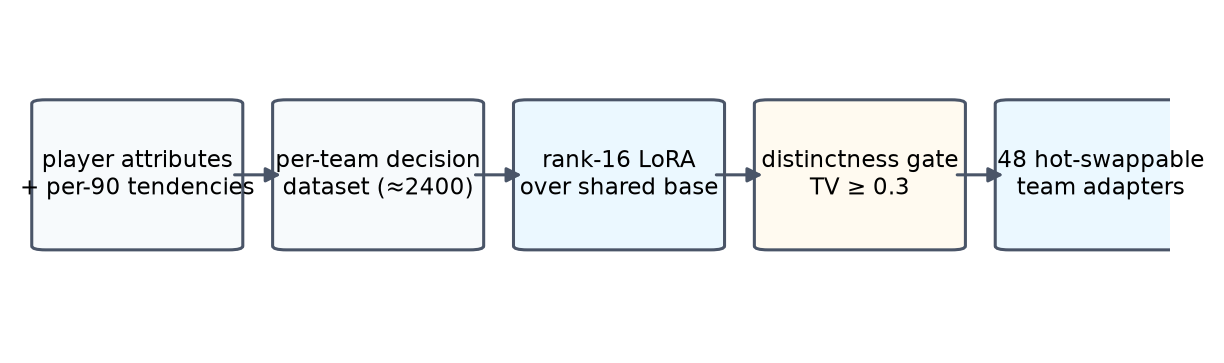
\includegraphics[width=0.96\textwidth]{fig_lora_pipeline.png}
\caption{Per-team identity pipeline. Player attributes and per-90-minute statistical tendencies are distilled into a team-specific decision dataset ($\approx2400$ examples), used to train a rank-$16$ LoRA over one shared base policy; the resulting per-team policy is admitted only if it clears a behavioural distinctness gate. Forty-eight national teams each become one hot-swappable adapter.}
\label{fig:lora}
\end{figure}

\paragraph{From attributes to a decision dataset.} For each team we synthesise a supervised dataset ($\approx2400$ examples) of (world-map context, decision) pairs. The decisions are generated from a team's players' attributes --- finishing, passing, tackling, pace, and role --- and from per-90-minute statistical tendencies (how often the team shoots, dribbles, presses), so that, e.g., a high-finishing forward in the attacking third is taught to shoot more readily, and a high-pressing side is taught to commit to tackles sooner. Each example is a short structured prompt (the coarsened context) and a target decision in the system's action vocabulary.

\paragraph{Low-rank adaptation over a shared base.} Each team $\tau$ is a low-rank adapter \citep{hu2021}: a base weight $W_0$ becomes $W_0+B_\tau A_\tau$ with $A_\tau\in\mathbb R^{r\times d}$, $B_\tau\in\mathbb R^{d\times r}$, rank $r=16\ll d$, trained by supervised fine-tuning on the team's dataset while the base is frozen. Two properties make this the right tool. First, \emph{cost}: a rank-$16$ adapter is a few tens of megabytes, so all forty-eight national teams fit alongside one shared base and are hot-swapped at serve time --- a fixture is selected by loading two adapters, not two models. Second, \emph{parsimony}: identity is a \emph{perturbation} of a shared footballing prior, not a separate model, which both regularises (the base supplies the common competence) and makes ``style'' a low-dimensional object we can reason about (\S\ref{sec:ident}).

\paragraph{A distinctness gate.} A team adapter is admitted to deployment only if it is behaviourally \emph{distinct}: on a fixed probe set of contexts, its decision distribution must differ from every other team's by at least a margin (a total-variation distinctness of $0.3$). This gate, analysed in \S\ref{sec:ident}, guarantees that the forty-eight adapters span genuinely different play styles rather than collapsing back onto the shared base.

\section{Knowledge-graph tactical grounding}\label{sec:kgsec}

Per-team LoRA encodes \emph{who} the players are; it does not, on its own, encode \emph{how the team intends to play} as a unit, nor does it let a designer state and edit tactics. \sfas{} supplies that layer with a \emph{tactical knowledge graph}, and --- as we argue below --- the knowledge graph is not a cosmetic add-on but the component that makes per-team LoRA and the message-free agent framework work better \emph{together} than either does alone (Fig.~\ref{fig:kg}).

\begin{figure}[t]\centering
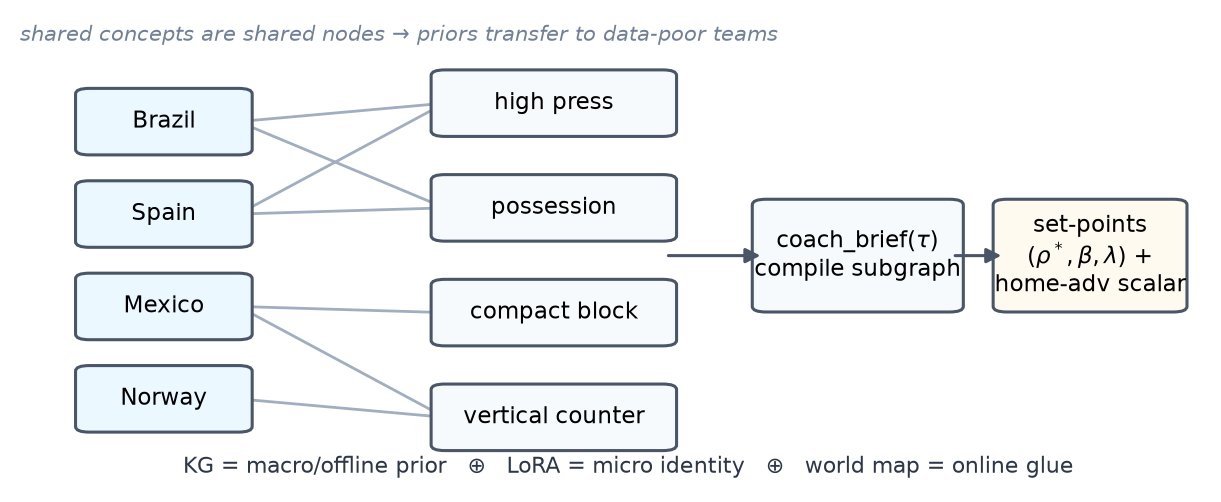
\includegraphics[width=0.98\textwidth]{fig_kg.png}
\caption{The knowledge graph and its synergy. \textbf{(1)} A relational graph links the forty-eight teams to shared tactical \emph{concepts} (high press, possession, compact block, vertical counter); teams that share a style share a node, so tactical knowledge \emph{transfers} and a data-poor team inherits priors through its neighbours. A per-team query \texttt{coach\_brief}$(\tau)$ compiles the relevant subgraph into control set-points $(\hat\rho,\beta,\lambda)$ and a home-advantage scalar (the schematic writes the possession target as $\rho^\star$; it is the compiled target $\hat\rho$ of \S\ref{sec:poss}, distinct from the feedback deadband $\rho^\star$). \textbf{(2)} These set-points are exactly what the control laws of \S\ref{sec:why} enforce, what the per-team LoRA's micro-decisions operate \emph{within}, and what aligns the otherwise message-free agents. The three layers are complementary: macro/offline prior $\oplus$ micro identity $\oplus$ online glue.}
\label{fig:kg}
\end{figure}

\subsection{What the graph is and how it works}

The graph is a relational tactical ontology over all forty-eight teams: nodes are teams, tactical \emph{concepts} (e.g.\ high pressing, possession retention, vertical counter-attack, compact mid-block), key player roles, and characteristic combinations; edges connect a team to the concepts it embodies and connect concepts that co-occur. Crucially, a tactical concept shared by several teams is \emph{one} node with multiple incident teams, so the graph is densely interconnected rather than forty-eight disjoint profiles. A lightweight, deterministic compilation turns each team's attributes and style descriptors into this graph; an optional language-model pass enriches it with narrative tactical text that is then indexed for hybrid (dense $+$ sparse) retrieval, in the manner of retrieval-augmented and graph-based RAG systems \citep{lewis2020,edge2024graphrag}.

At match time a single read, $\texttt{coach\_brief}(\tau)$, retrieves the subgraph around team $\tau$ --- its concepts, its salient combinations, and, through the shared-concept edges, the tactical neighbourhood it sits in --- and compiles it into the handful of \emph{control set-points} the rest of the system consumes: a possession target (which enters the \emph{fixture} anchor of \S\ref{sec:why}, compiled from \emph{both} teams' style vectors by the learned calibration policy), a pressing level (which sets the reinforcement/turnover regime $\beta$), and a shape tightness (which informs the anchoring weight $\lambda$). The read is offline and self-contained --- no live database is needed inside the match loop --- so the graph adds tactical grounding without adding runtime coupling.

\subsection{How it improves the system}

Grounding tactics in a graph rather than in a free-text prompt buys four things. \emph{(i) Consistency:} the same tactical facts are injected every match, so a team's macro-behaviour is reproducible rather than re-sampled from a prompt each time. \emph{(ii) Transfer:} because shared styles are shared nodes, a team with little training data inherits tactical priors from its better-attested neighbours --- the graph generalises across teams in a way a per-team artifact cannot. \emph{(iii) An interpretable, editable interface:} a designer states ``this side presses high and keeps the ball,'' edits one node, and the change propagates deterministically into the control set-points --- tactics are inspectable and version-controlled, not buried in weights. \emph{(iv) Separation of concerns:} the graph carries \emph{team-level intent} while the LoRA carries \emph{player-level tendency}, so the two can be developed, validated and swapped independently.

\subsection{Synergy with LoRA and the agent framework}

The three components operate at different levels and reinforce one another (Fig.~\ref{fig:kg}, right); this is the heart of why the combination works.

\paragraph{Graph $\oplus$ LoRA: macro intent meets micro identity.} The LoRA shifts a player's \emph{micro} decision distribution (a high-finishing striker shoots sooner); the graph sets the \emph{macro} envelope the team plays within (press high, target $59\%$ possession). Neither subsumes the other: a possession-style set-point with a route-one striker's adapter produces patient build-up that still ends in early shots, a combination no single prompt reliably elicits. The graph also \emph{compensates for the LoRA's data limits}: where a small federation's adapter is thin, the shared-concept edges transfer a sensible tactical prior, so the team is coherent even when its micro-policy is undertrained. Concretely, the graph chooses the target $\hat\rho$ and the $\beta,\lambda$ set-points; the LoRA chooses the per-frame action \emph{distribution} conditioned on those; the calibration gate (\S\ref{sec:calib}) checks the joint result.

\paragraph{Graph $\oplus$ agent framework: the team-level correlation device.} The agents are message-free (Prop.~\ref{prop:factor}): within a frame they coordinate only through the shared world map, which carries \emph{positional} but not \emph{strategic} common knowledge. There is therefore no in-match channel by which eleven teammates could agree to, say, press high as a unit. The knowledge graph fills exactly this gap: it is an \emph{offline, team-level correlation device}, a manager's pre-match instruction internalised by every agent on the side through the shared set-points, where the world map is the \emph{online, frame-level} correlation device. The two correlation devices act on different time-scales and are complementary --- without the graph the agents would be positionally but not tactically coordinated; without the shared map they could not execute the tactics frame-to-frame. In the language of \S\ref{sec:why}, the graph sets the \emph{set-points}, the world map carries the \emph{state}, the LoRA supplies the \emph{policy}, and the control laws of \S\ref{sec:why} guarantee the emergent result is stable. This division of labour --- macro/offline prior $\oplus$ micro identity $\oplus$ online glue, all kept honest by an outer calibration loop --- is the core architectural idea of \sfas.

\section{Why the system is stable}\label{sec:why}

This section explains the two failure modes of \S\ref{sec:intro} and the control laws that cure them. We keep statements in the main text and defer full proofs to Appendix~\ref{app:proofs}; the emphasis here is on the mechanism and on the figures.

\subsection{Coordination without communication}\label{sec:stig}

A \emph{stigmergic Markov game} is a Markov game in which every agent observes the same map $w_t=\Wmap(s_t)$, has no other input (no communication, no peek at others' actions or memory within a frame), and the state advances by a fixed operator $s_{t+1}=\Phi(s_t,\mathbf a_t)$.

\begin{proposition}[policy factorisation]\label{prop:factor}
In a stigmergic Markov game the joint action distribution factorises over agents conditional on the world map, $\Prob(\mathbf a_t\mid s_t)=\prod_{i=1}^{22}\pi_i(a_i\mid\Wmap(s_t))$, so the one-step transition is $\Prob(s_{t+1}\mid s_t)=\sum_{\mathbf a}\mathbf1\{s_{t+1}=\Phi(s_t,\mathbf a)\}\prod_i\pi_i(a_i\mid\Wmap(s_t))$. All cross-agent dependence in the realised trajectory is generated by $\Phi$ and the recursion; none within a decision step. The shared map acts as a correlation device.
\end{proposition}

This is the formal license for the parallel, message-free serving of \S\ref{sec:serve}, and it tells us where coordination failures live: not in any single $\pi_i$, but in the interaction of the product policy with $\Phi$ over time. The two pathologies below are exactly such interaction effects.

\subsection{Possession is bistable --- and a feedback law fixes it}\label{sec:poss}

Let $b_t\in\{0,1\}$ indicate home holds the ball at frame $t$ (loose-ball frames excluded). The system tracks home's \emph{recent possession share} by an exponentially weighted estimator with weight $\alpha$,
\begin{equation}\label{eq:ema}
\rho_{t+1}=(1-\alpha)\rho_t+\alpha\,b_{t+1},\qquad\rho_0=\tfrac12 .
\end{equation}
Because the dominating team keeps its shape and press, the probability it wins the next duel rises with its recent share; we capture this by turnover hazards $h_H(\rho)=h_0e^{-\beta(2\rho-1)}$, $h_A(\rho)=h_0e^{+\beta(2\rho-1)}$, so the next-holder probability is $q(\rho)=h_A/(h_A+h_H)=\sigma(4\beta(\rho-\tfrac12))$ with logistic $\sigma$ and \emph{reinforcement strength} $\beta\ge0$. The asymptotics of the frame-indexed process \eqref{eq:ema} are governed by a one-dimensional mean field.

\begin{lemma}[mean-field reduction]\label{lem:meanfield}
The recent-share process \eqref{eq:ema} is a constant-gain Robbins--Monro recursion whose mean field is the gradient flow
\begin{equation}\label{eq:meanode}
\dot\rho=m(\rho):=q(\rho)-\rho=\sigma\!\big(4\beta(\rho-\tfrac12)\big)-\rho .
\end{equation}
With probability one the interpolated trajectory of $\{\rho_t\}$ converges to the set of fixed points of $m$ and cannot converge to a linearly unstable one; around a stable fixed point $\rho^\ast$ its stationary fluctuation has variance $\alpha\,q(\rho^\ast)(1-q(\rho^\ast))/(2|m'(\rho^\ast)|)+O(\alpha^2)$, i.e.\ an $O(\sqrt\alpha)$ band.
\end{lemma}

\noindent (Proof in Appendix~\ref{app:proofs}, by the stochastic-approximation ODE method \citep{benaim1999,kushner2003}.) The stability of the equilibria of $m$ therefore determines the emergent possession; we analyse it now.

\begin{theorem}[bistability of emergent possession]\label{thm:bistable}
The balanced state $\rho=\tfrac12$ is a fixed point of $\dot\rho=m(\rho)$, linearly stable iff $\beta<1$. As $\beta$ crosses $1$ the system undergoes a supercritical pitchfork: for $\beta>1$ the balanced state is unstable and two stable fixed points $\rho_\pm(\beta)$ appear, with $\rho_\pm\to\{0,1\}$ as $\beta\to\infty$. Hence for any $\beta>1$ the uncontrolled simulator drives possession to a near-monopoly almost surely (Fig.~\ref{fig:bif}).
\end{theorem}

Theorem~\ref{thm:bistable} (Fig.~\ref{fig:bif}) is the exact statement of the snowball: whenever holding the ball is even mildly self-reinforcing, an \emph{uncontrolled} simulator \emph{must} drive possession to a monopoly, the winner decided by early noise. No prompt engineering removes this; it is a property of the mean field and must be cured in the dynamics.

\begin{figure}[t]\centering
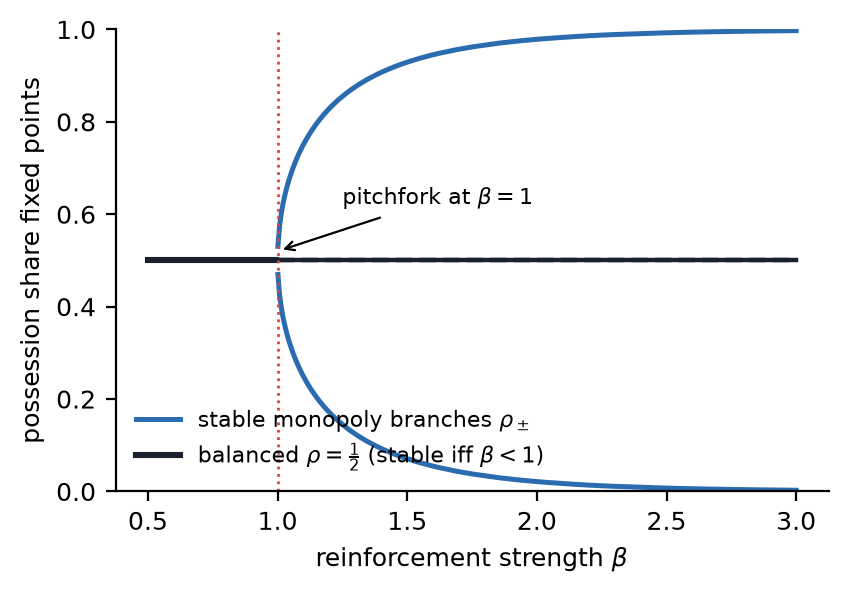
\includegraphics[width=0.72\textwidth]{fig_bifurcation.png}
\caption{The open-loop possession mean field undergoes a supercritical pitchfork at reinforcement strength $\beta=1$: the balanced $50\%$ equilibrium (stable for $\beta<1$) loses stability, and two stable possession-monopoly branches emerge --- the snowball failure mode (Thm.~\ref{thm:bistable}).}
\label{fig:bif}
\end{figure}

The cure is a feedback that \emph{opposes} dominance: once a team's recent share passes a deadband $\rho^\star$, inflate \emph{its} turnover hazard in proportion to the excess, $h_H(\rho)\mapsto h_H(\rho)(1+g(\rho-\rho^\star)_+)$ and symmetrically for away, with \emph{feedback gain} $g\ge0$.

\begin{theorem}[stabilisation and the critical gain]\label{thm:stabilise}
Let $\beta>1$ and $\rho^\star=\tfrac12$. Under the feedback the balanced state is a fixed point of the controlled mean field, linearly stable iff
\begin{equation}\label{eq:gstar}
g>g^\star=4(\beta-1).
\end{equation}
For $g>g^\star$ it is the \emph{unique} stable equilibrium, the monopolies $\rho_\pm$ are destroyed, and the closed-loop possession \eqref{eq:ema} concentrates in an $O(\sqrt\alpha)$ neighbourhood of the target.
\end{theorem}

Equation~\eqref{eq:gstar} is the central practical statement: make the anti-dominance gain larger than four times the excess reinforcement, and a guaranteed monopoly becomes a controlled, realistic match. The system uses $g=22$, $\alpha=0.02$ (a $\approx50$-frame window) and $\rho^\star=0.55$; $g=22$ clears $g^\star$ for every $\beta$ up to $6.5$ --- a wide margin over the realistic regime --- and the small $\alpha$ gives the $O(\sqrt\alpha)\approx0.14$ single-match fluctuation band we observe. Figure~\ref{fig:feedback} confirms the bifurcation and its removal directly by Monte-Carlo of \eqref{eq:ema}: with $g=0<g^\star$ the final-possession histogram is bimodal at the monopolies; with $g=22>g^\star$ it is unimodal at the set-point.

\begin{figure}[t]\centering
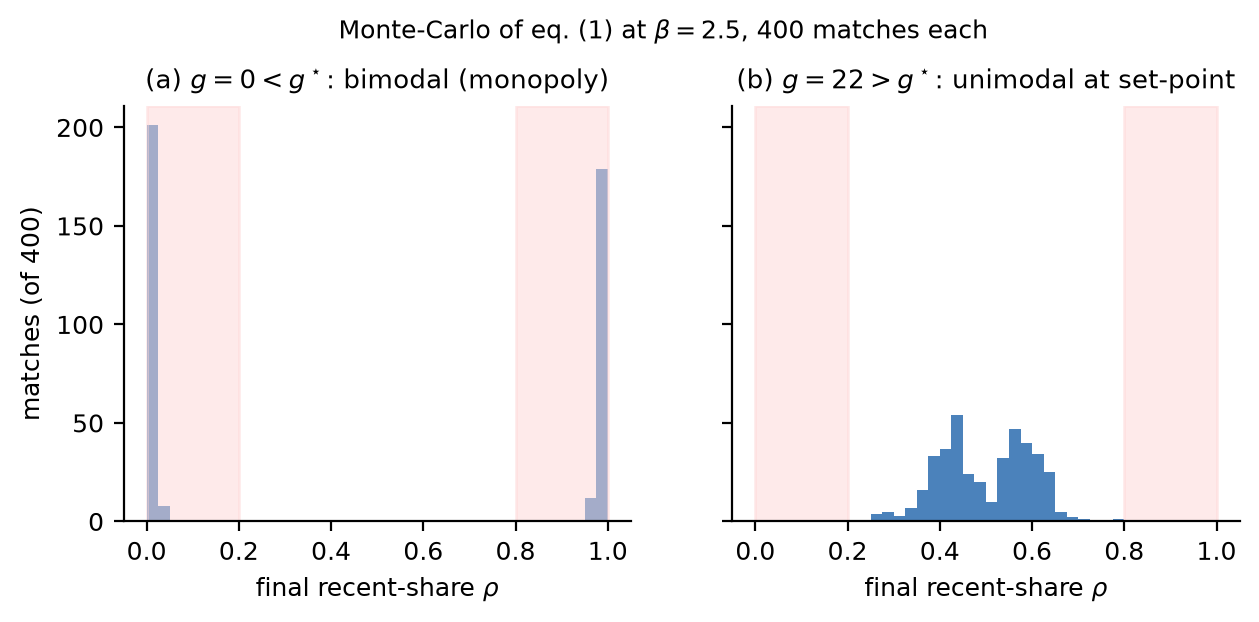
\includegraphics[width=0.92\textwidth]{fig_feedback.png}
\caption{Monte-Carlo of the possession process \eqref{eq:ema} at $\beta=2.5$ ($400$ matches each). (a) Without feedback ($g=0<g^\star$) final possession is bimodal --- the team that leads early monopolises the ball. (b) With feedback ($g=22>g^\star$) it is unimodal and concentrated at the set-point, exactly as Theorem~\ref{thm:stabilise} predicts.}
\label{fig:feedback}
\end{figure}

\begin{corollary}[home-advantage set-point]\label{cor:setpoint}
A small home edge $h_H\mapsto h_H(1-\eta_H)$, $h_A\mapsto h_A(1+\eta_A)$ moves the unique stable fixed point to $\rho^\dagger=\tfrac12+(\eta_H+\eta_A)/(2(g-g^\star))+O(\eta^2)$. A single home-advantage scalar thus shifts the calibrated possession target continuously and monotonically.
\end{corollary}

Corollary~\ref{cor:setpoint} is the bridge from the knowledge graph to the physics: a tactical instruction (``dominate possession'') maps to a desired share, which maps through the monotone relation above to one scalar, which Theorem~\ref{thm:stabilise} then holds in place. \emph{The graph sets the set-point; the control law enforces it.}

\paragraph{Matchup-dependent calibration, learned rather than hand-set.} The corollary's set-point is not a global constant: it is compiled \emph{per fixture} from both teams' real style vectors (a 48-team library of measured possession, pass-completion and strength statistics). The compiled target is
\[
\hat\rho(h,a)=\operatorname{clip}\!\big(\tfrac12+\kappa\,[\,w_p\Delta_{\mathrm{poss}}+w_c\Delta_{\mathrm{pass}}+w_z\Delta_z\,]+\eta_{\mathrm{home}},\ \tfrac12\pm b\big),\qquad b=0.065,
\]
realised through Corollary~\ref{cor:setpoint} as the closed-loop fixed point $\rho^\dagger$ --- so Spain--Austria and Brazil--Japan receive \emph{different} calibrations while no two fixtures' targets may diverge by more than $13$ points. Enforcement is deliberately soft --- \emph{guided emergence}: the target sets a low-gain director ($k_p=0.4$, a coach's nudge rather than a pull) and a weakened physical lean, while three style channels enter as \emph{behavioural} modifiers --- pressing scales the opponent's turnover hazard by $(1+0.6\,(\mathrm{press}-\tfrac12))$ and tightens marking distances by $(1-0.30\,(\mathrm{press}-\tfrac12))$ inside the contextual pass-completion model; tempo scales the holder's release hazard; directness rescores pass-target selection --- so the possession difference \emph{emerges from the behavioural contest} rather than being imposed. The split of labour is visible in the numbers: for the heaviest mismatches the compiled target saturates at the clip ($56.5\%$) while the emergent seat is $68.2$--$68.6\%$ (\S\ref{sec:exp}) --- the target contributes at most $6.5$ points of the seat, and the remaining $\approx12$ points are produced by the behavioural channels acting through the contest. The eight calibration parameters $\theta=(\kappa,w_p,w_c,w_z,\text{lean scale},\text{three style gains})$ are \emph{learned} by cross-entropy-method policy search \citep{rubinstein2004} over engine rollouts, with per-fixture loss $|\text{emergent share}-\text{real-world anchor}|$ plus a monopoly penalty and a pass-completion band penalty. Training uses three strength-diverse fixtures --- \emph{Spain--Austria}, \emph{Brazil--Japan} and an off-corpus \emph{Qatar--Spain} --- so \emph{five of the seven evaluation fixtures are held out}, including both heavy mismatches (\emph{Argentina--Cape Verde}, \emph{Paraguay--France}) behind the venue-symmetry check; the loss falls $0.232\to0.150$ in four iterations (population $8$), giving $\kappa=1.18$, $w_p=0.44$, $w_c=0.11$, $w_z=0.01$ and press/directness/tempo gains $0.69/0.38/0.50$ (policy archived in \texttt{calib\_policy.json}; trainer \texttt{calibrate\_policy.py}). That the learned target leans on style deltas rather than the raw strength difference ($w_z\approx0$) is expected --- possession and passing styles already encode strength --- so the strength-gap scaling of \S\ref{sec:exp} is carried through the style channels rather than a separate strength term. The two observables of \S\ref{sec:exp} --- the dominant side's seat scaling smoothly with the strength gap, and its venue symmetry ($68.2\%$ home vs $68.6\%$ away, both on held-out fixtures) --- follow from this fixture-dependent, learned policy: the target \emph{plus} the behavioural gains, not the target alone.

\begin{remark}[deadband, operating point, and inferring $\beta$]\label{rem:deadband}
Theorem~\ref{thm:stabilise} analyses the symmetric deadband $\rho^\star=\tfrac12$, for which the threshold is exactly $g^\star=4(\beta-1)$. The deployed system uses $\rho^\star=0.55$: inside $[1-\rho^\star,\rho^\star]$ the feedback is inactive, so the balanced state is \emph{locally} unstable (the open-loop slope $m'(\tfrac12)=\beta-1>0$) and the share drifts outward until, at the band edge, the feedback engages and arrests it. The stable operating point therefore sits just outside the deadband, near $\rho^\star$ --- which is why, in deployment, fixtures seat within a few points of their compiled targets --- Brazil--Japan (target $55\%$) just past the band edge at $59\%$, C\^ote d'Ivoire--Norway ($53\%$) at $52\%$, Mexico--Ecuador ($50\%$) at $54\%$ (Cor.~\ref{cor:setpoint}). We \emph{measure} the reinforcement from six open-loop ($g=0$) ablation matches ($4{,}325$ held ticks; $36$ window-transition pairs at $W=100$). The primary evidence of supercriticality is behavioural (Fig.~\ref{fig:betaabl}): five of the six matches drift to the extremes --- $69\%$ of share windows fall at $\rho\le0.35$ or $\rho\ge0.65$ and only $5\%$ remain central, with leading modal share $\rho^+=0.68$ --- whereas the closed loop on balanced fixtures is unimodal ($11\%$ extreme, $33\%$ central); by Theorem~\ref{thm:bistable} read in reverse, such drift occurs only for $\beta>1$. Point estimates agree in sign: the local slope of the share-transition map $q(\rho)=\sigma(4\beta(\rho-\tfrac12))$ at $\rho^\star=\tfrac12$ (the direct estimator) gives $\hat\beta\approx1.6$--$2.3$, and the modal fixed-point relation $\beta=\operatorname{logit}(\rho^+)/\big(4(\rho^+-\tfrac12)\big)$ gives $\hat\beta\approx1.05$; a \emph{global} logistic fit yields $0.77$--$0.91$, an underestimate by construction here since it pools the saturated branches where the drift is clipped (the same mechanism that makes the AR(1) slope a lower bound, $\approx0.7$--$0.8$). A synthetic recovery study (the same estimator pipeline on trajectories generated from the share-transition map $q(\rho)$ with known $\beta$; archived in \texttt{beta\_estimator\_calibration.txt}) confirms this reading: AR(1) returns $<1$ even at true $\beta=2$ ($0.93$--$1.00$); under engine-like branch saturation the modal estimator compresses to $\approx1.05$ \emph{regardless} of true $\beta\in[1.5,2]$ --- matching our measured $1.047$ --- while a subcritical control ($\beta=0.8$) yields only $29$--$38\%$ extreme windows and local slope $<1$, versus $83$--$100\%$ and $\approx1.9$ when supercritical (measured: $69\%$ and $1.6$--$2.3$). The data are thus consistent with a genuinely supercritical system and inconsistent with a subcritical one. The conclusion is insensitive to this spread: even the largest estimate gives $g^\star=4(\hat\beta-1)\approx5.1$, and the deployed $g=22$ clears $g^\star$ for every $\beta$ up to $6.5$ --- the feedback sits far above the critical gain, which is why closed-loop possession seats firmly in band (\S\ref{sec:exp}).
\end{remark}

\begin{figure}[t]\centering
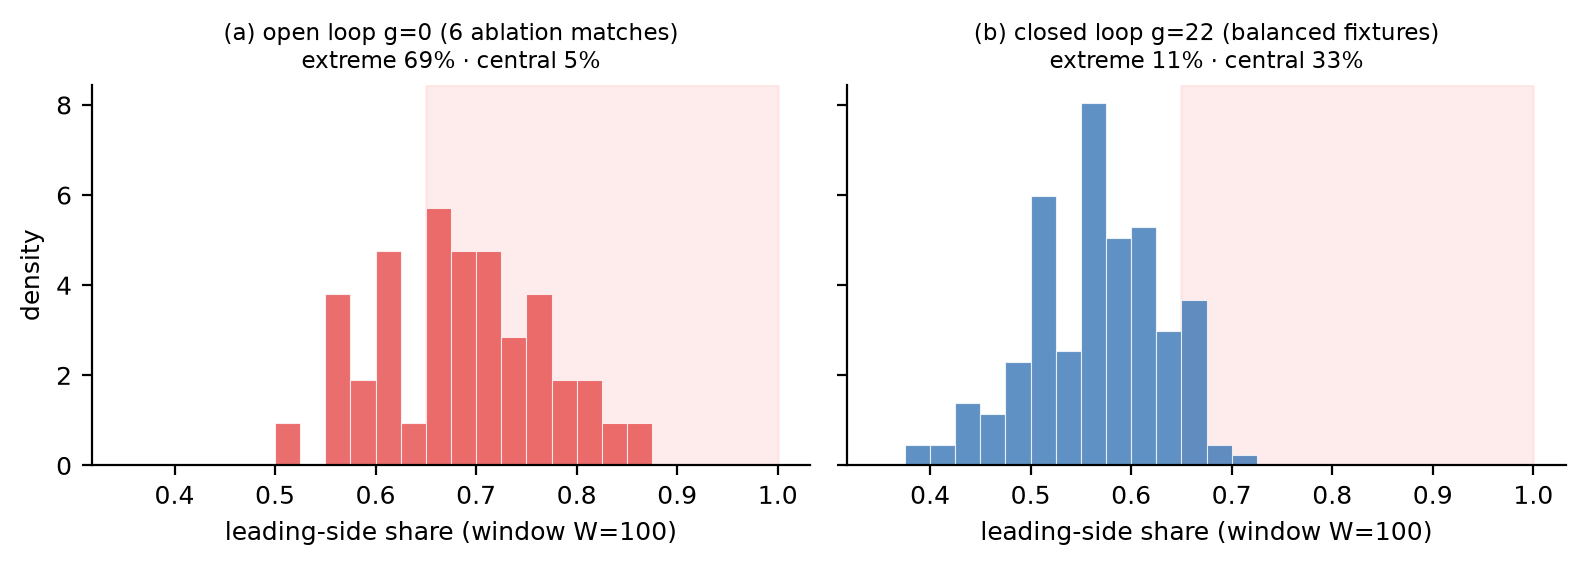
\includegraphics[width=0.94\textwidth]{fig_beta_ablation.png}
\caption{Leading-side share distributions (windows of $W=100$ held frames). (a) Open loop ($g=0$, six ablation matches): mass drifts to the extremes --- $69\%$ of windows at $\rho\le0.35$ or $\rho\ge0.65$, only $5\%$ central --- the bimodal signature Theorem~\ref{thm:bistable} predicts for $\beta>1$. (b) Closed loop ($g=22$, the two balanced fixtures): unimodal, $11\%$ extreme / $33\%$ central; the monopoly zone (shaded) stays empty.}
\label{fig:betaabl}
\end{figure}

\subsection{Formations cannot collapse}\label{sec:collapse}

Off the ball each agent emits a target $z_i^t$; followed literally, ``go to the ball'' collapses the shape. The resolution operator instead moves each player towards a \emph{convex blend} of its target and a fixed formation anchor $\phi_i$, with step $\eta$ and blend weight $\lambda$:
\begin{equation}\label{eq:anchor}
x_i^{t+1}=(1-\eta)x_i^t+\eta\big[(1-\lambda)\phi_i+\lambda z_i^t\big].
\end{equation}

\begin{proposition}[non-collapse guarantee]\label{prop:noncollapse}
Let every agent target a common point (the worst case, e.g.\ all chase the ball), with bounded idiosyncratic heterogeneity of cross-player variance $\sigma_z^2$. Then the stationary formation dispersion of \eqref{eq:anchor} is $S_\infty^2=(1-\lambda)^2S^2+\lambda^2\sigma_z^2\ge(1-\lambda)^2S^2$, where $S^2$ is the dispersion of the formation anchors. Hence for any $\lambda<1$ the formation cannot collapse; collapse requires $\lambda=1$ and $\sigma_z=0$, a measure-zero case.
\end{proposition}

Proposition~\ref{prop:noncollapse} (Fig.~\ref{fig:disp}) turns the design constant $\lambda<1$ into a guarantee and quantifies the trade-off: larger $\lambda$ gives agents more authority over shape (more tactical expressiveness) at the cost of a smaller guaranteed spread $(1-\lambda)^2$. \sfas{} anchors twice (a $\lambda_1=0.45$ blend when the intent is formed and a further $\lambda_2=0.40$ in the motion model), so the retained-structure factors multiply to $((1-\lambda_1)(1-\lambda_2))^2\approx0.11$: even under universal ball-chasing the team keeps $\approx11\%$ of its formation spread, which prevents the degenerate ``all twenty-two on the ball'' state while still letting tactics deform the shape.

\begin{figure}[t]\centering
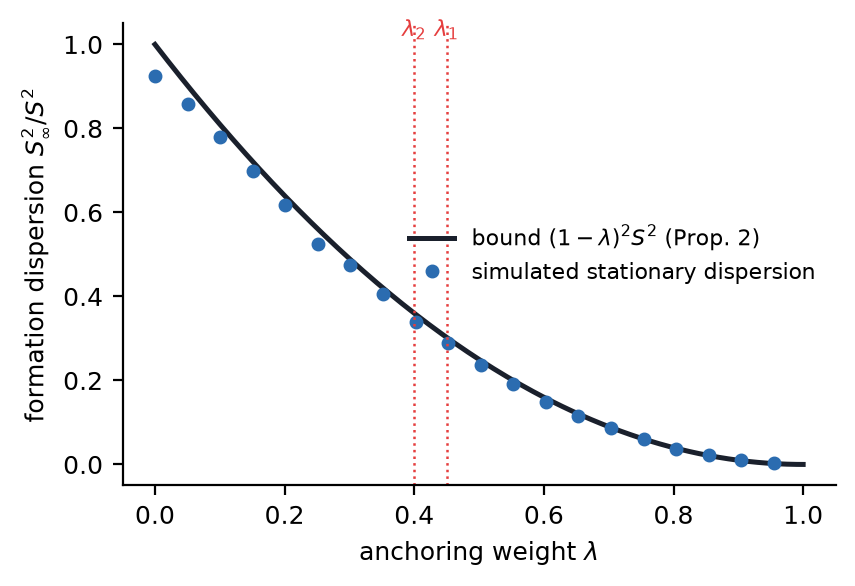
\includegraphics[width=0.66\textwidth]{fig_dispersion.png}
\caption{Intent anchoring guarantees a positive lower bound $(1-\lambda)^2S^2$ on formation dispersion for any blend weight $\lambda<1$ (Prop.~\ref{prop:noncollapse}); collapse is possible only in the boundary case $\lambda=1$. \sfas{}'s two-stage anchoring keeps $\approx11\%$ of the formation spread even when all agents chase the ball.}
\label{fig:disp}
\end{figure}

\subsection{Calibration as an outer loop}\label{sec:calib}

The control laws above are tuned so that the \emph{aggregate} statistics land in independently specified realism bands (Table~\ref{tab:bands}). Two couplings matter. The possession band \emph{and} the number of possession sequences are both governed by Theorem~\ref{thm:stabilise} --- the fixed point sets the mean share, and the turnover hazard at that point sets how often possession changes. And the shot statistics are meaningful only because Proposition~\ref{prop:noncollapse} keeps the formation from collapsing; a collapsed shape would manufacture or suppress shots unphysically. Calibration is thus not eleven independent tunings but a few identified laws whose parameters the bands pin down.

\begin{table}[h]\centering
\caption{Realism bands enforced by the calibration gate (per-team, per-match unless noted), and the governing law. Bands are reference ranges for \emph{typical} matches, consistent with public match data (Opta/FBref) and the 2022 World Cup; legitimate extremes lie beyond them --- elite possession sides reach $\sim$70--80\% (e.g.\ Spain at the World Cup) and deep blocks fall below $30\%$, while per-match ratios over few attempts (save rate, shots-on-target\%) have heavy tails (\S\ref{sec:exp}).}
\label{tab:bands}
\small
\begin{tabular}{lcc}
\toprule
Statistic & Realism band & Governing law \\
\midrule
Possession share & $30$--$70\%$ & Thm.~\ref{thm:stabilise}, Cor.~\ref{cor:setpoint} \\
Shots & $5$--$20$ & shot gate $+$ dispersion (Prop.~\ref{prop:noncollapse}) \\
Shots on target & $25$--$50\%$ & finishing contest \\
Save rate & $60$--$80\%$ & goalkeeper contest \\
Pass completion & $50$--$90\%$ & contextual interception (measured per-attempt) \\
Offside frequency & $0$--$5$ & line geometry \\
Possession sequences & $60$--$220$ & Thm.~\ref{thm:stabilise} (turnover rate) \\
Goals & $0$--$7$ & finishing contest (Skellam diff.\ \citep{skellam1946}) \\
Expected goals (xG) & consistency with goals & shot-quality model \\
Recovery time (s) & $5$--$60$ & turnover hazard \\
\bottomrule
\end{tabular}
\end{table}

\section{Experiments}\label{sec:exp}

\paragraph{Setup.} Team adapters are distilled at rank $r=16$ over one shared base policy from per-team decision datasets ($\approx2400$ examples each) for the forty-eight finalists of the 2026 World Cup. Per-fixture possession anchors are compiled from both teams' real style vectors by the learned calibration policy of \S\ref{sec:why} (CEM-fitted, archived in \texttt{calib\_policy.json}) and enforced softly ($k_p=0.4$ director, weakened lean, style$\to$behaviour gains). Each match runs $\approx4000$ frames (ninety-minute equivalent); the on-ball brain is a single shared model --- run here as \emph{Nemotron-3 Super} and, on a second machine, as \emph{Qwen3.5-35B-A3B}, with consistent behaviour --- and the two off-ball policies are \emph{Gemma-4-E2B} adapters served as independent daemons (\S\ref{sec:serve}); the backbone is interchangeable. Every match is archived with its full per-frame trajectory, eleven-statistic line, run configuration and an animated replay; all figures below are reproducible from the corpus. The corpus is $75$ matches over seven fixtures spanning the strength spectrum: \emph{Brazil}--\emph{Japan}, \emph{C\^ote d'Ivoire}--\emph{Norway}, \emph{Mexico}--\emph{Ecuador}, \emph{Spain}--\emph{Austria}, \emph{Belgium}--\emph{Senegal} and \emph{Argentina}--\emph{Cape Verde} (ten matches each), plus a fifteen-match \emph{Paraguay}--\emph{France} series. Because every match is archived in the same schema, extending the corpus is purely additive and changes no part of the system.

\paragraph{Statistical realism (Fig.~\ref{fig:bands}).} Across all $75$ matches the aggregate statistics sit inside their realism bands. Pass completion is in-band in all $150$ team-matches ($64.6$--$87.4\%$, mean $76.3\%$); the dominant side's possession scales with the strength gap (per-fixture means $52$--$60\%$ from the balanced to the intermediate pairs, up to $68$--$69\%$ for the heavy mismatches) and stays inside $30$--$70\%$ in every match; sequences, offsides and recovery track their bands; goals and xG are consistent ($149$ goals vs $207$ xG, $-0.39$ goals$-$xG per team-match --- finishing is noisy and slightly conservative). Two understood per-match exceptions remain. The first is the shot count, which exceeds the conservative $5$--$20$ band in the highest-tempo matches --- faithful to real football, where open games produce $25+$ shots --- and falls below it for the deepest defensive blocks in mismatches. The second is the save rate: as a ratio over the few shots on target in a single match it is intrinsically high-variance, and reaches $100\%$ in low-shot matches (a small-denominator effect, exactly as a real clean sheet does). Both are properties of per-match ratios over small counts, not of the dynamics; the season-style bands in Table~\ref{tab:bands} describe \emph{typical} values, which the means respect.

\begin{figure}[t]\centering
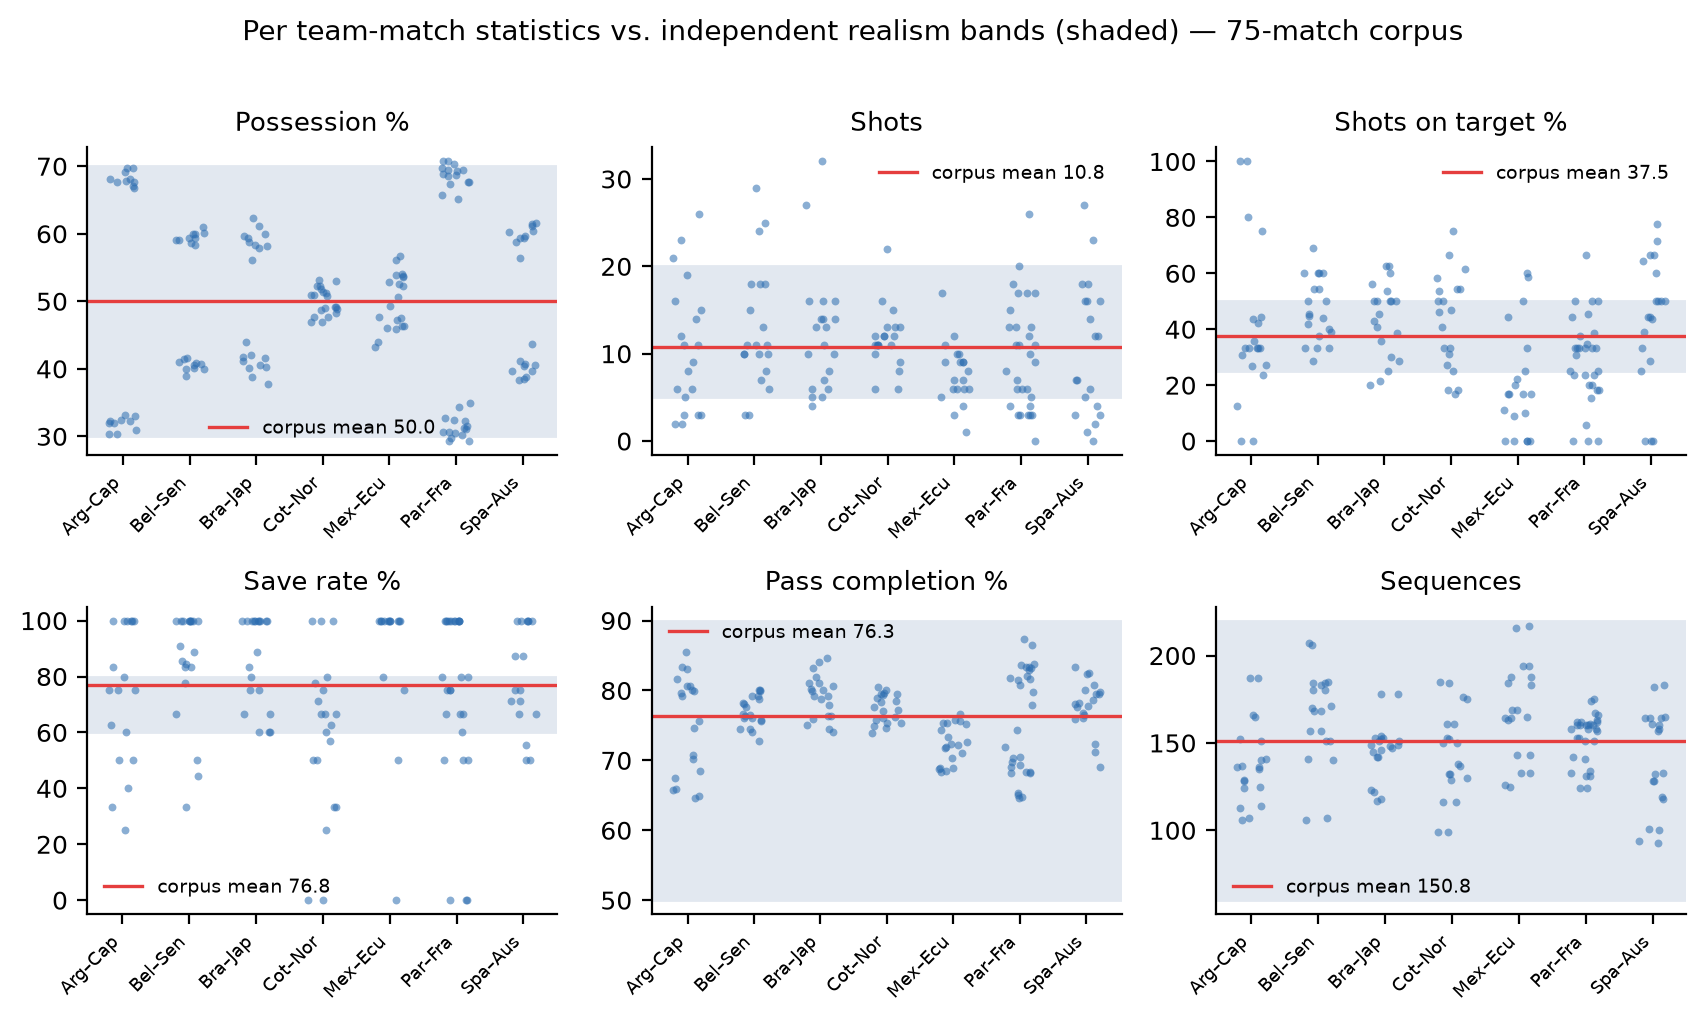
\includegraphics[width=0.94\textwidth]{fig_stat_bands.png}
\caption{Six representative aggregate statistics (of eleven) across the seven-fixture, $75$-match corpus, per team, against independent realism bands (shaded). Means lie inside every band; the shot-band excursions are the highest-tempo matches and the deepest defensive blocks.}
\label{fig:bands}
\end{figure}

\paragraph{Possession in action (Fig.~\ref{fig:timeline},~\ref{fig:poss}).} The closed loop is visible within a single match (Fig.~\ref{fig:timeline} --- the \emph{Paraguay}--\emph{France} $1$--$0$ upset): the dominant side's cumulative possession converges to $69.5\%$ while the recent-share EMA fluctuates around it and, after an early transient, \emph{never re-enters} the $>80\%$ monopoly region the open-loop dynamics drifts to --- the empirical face of Theorem~\ref{thm:stabilise}, in the hardest case (a heavy mismatch). Across all $75$ matches (Fig.~\ref{fig:poss}) the dominant side's seat scales smoothly with the strength gap --- $52$--$60\%$ in balanced fixtures, $65$--$70\%$ in the heaviest mismatches --- and never becomes a monopoly. Two checks close the loop: \emph{venue symmetry} --- the strong side seats at $68.2\%$ at home (Argentina) and $68.6\%$ away (France), a $0.5$-point difference, so the seat is strength, not venue --- and \emph{possession $\neq$ outcome}: France conceded $69.5\%$ possession and lost the displayed match.

\begin{figure}[t]\centering
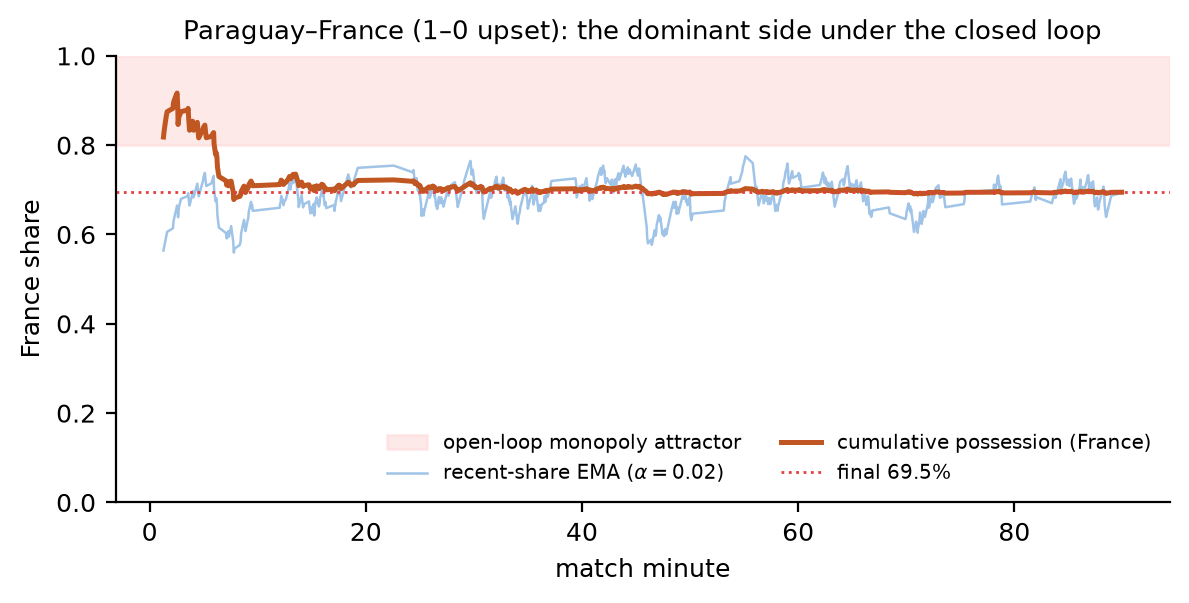
\includegraphics[width=0.86\textwidth]{fig_timeline.png}
\caption{The dominant side within one match (\emph{Paraguay}--\emph{France}, $1$--$0$ upset). France's cumulative possession (dark) converges to $69.5\%$; the recent-share EMA (light) fluctuates with the predicted $O(\sqrt\alpha)$ amplitude and, after the opening transient, stays out of the open-loop monopoly attractor (shaded) --- and France still loses. This is the closed loop of Theorem~\ref{thm:stabilise} in operation, in the hardest (heavy-mismatch) case.}
\label{fig:timeline}
\end{figure}

\begin{figure}[t]\centering
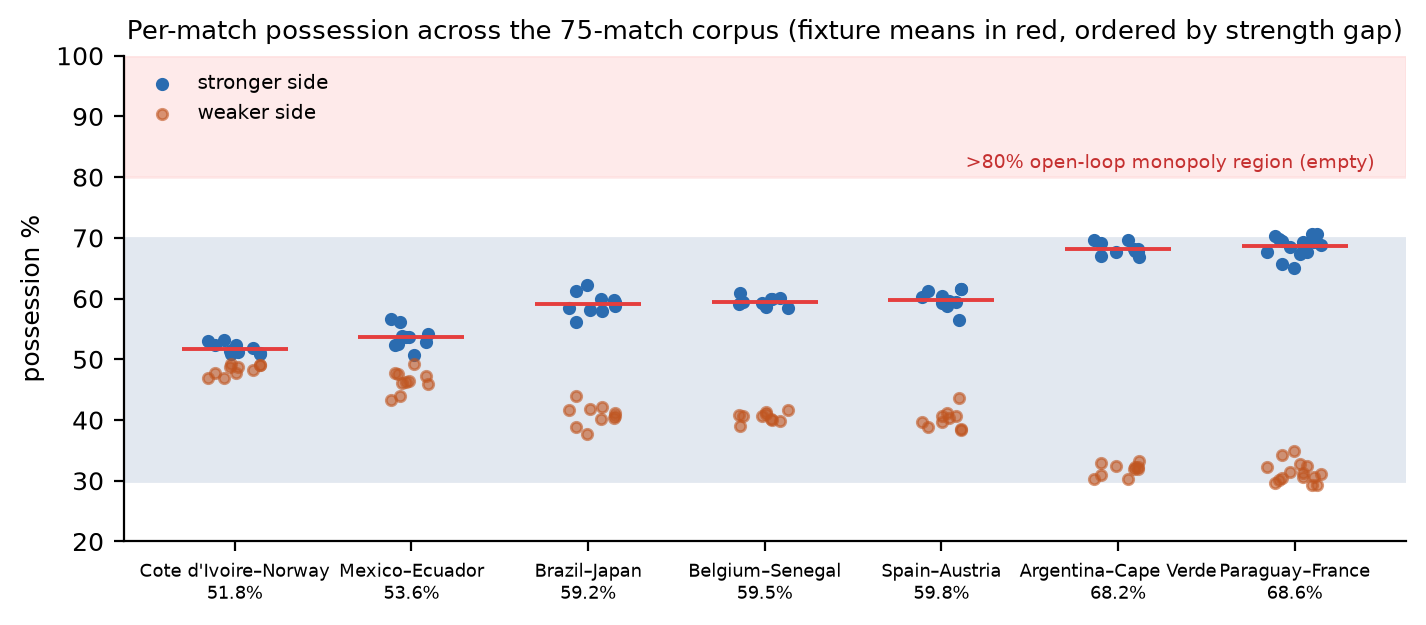
\includegraphics[width=0.84\textwidth]{fig_possession.png}
\caption{Per-match possession across all seven fixtures. The dominant side's seat scales with the strength gap; neither team ever approaches the monopoly region, and every match stays inside the $30$--$70\%$ realism band.}
\label{fig:poss}
\end{figure}

\paragraph{Competitive balance and finishing (Fig.~\ref{fig:results},~\ref{fig:shotsxg}).} Records track strength without becoming scripted (Fig.~\ref{fig:results}): the two balanced fixtures split (\emph{Brazil}--\emph{Japan} $3$-$4$-$3$, \emph{Mexico}--\emph{Ecuador} $2$-$6$-$2$), while the other five are \emph{one-sided} --- a side wins the series by six or more (Spain $7$-$2$-$1$, Belgium and Argentina $8$-$1$-$1$, C\^ote d'Ivoire $6$-$3$-$1$, France $8$-$5$-$2$ \emph{away}). Yet in those five one-sided fixtures the out-matched side (the series loser) still wins $6$ of $55$ matches ($11\%$), the realistic upset rate the stabilisation law makes possible: dominated sides stay in matches instead of being run over. Overall $36$-$22$-$17$ to the home side with $149$ goals and no blowout artefacts --- precisely the regime the stabilisation law is meant to protect, since an unstabilised simulator would let the possession monopolist run away. Shot volume tracks territorial control, and realised goals scatter around the expected-goals diagonal (Fig.~\ref{fig:shotsxg}) with a conversion slightly below one: finishing is noisy match-to-match, as in real football, and mildly conservative in aggregate. A representative match is detailed in Table~\ref{tab:bvj}.

\begin{figure}[t]\centering
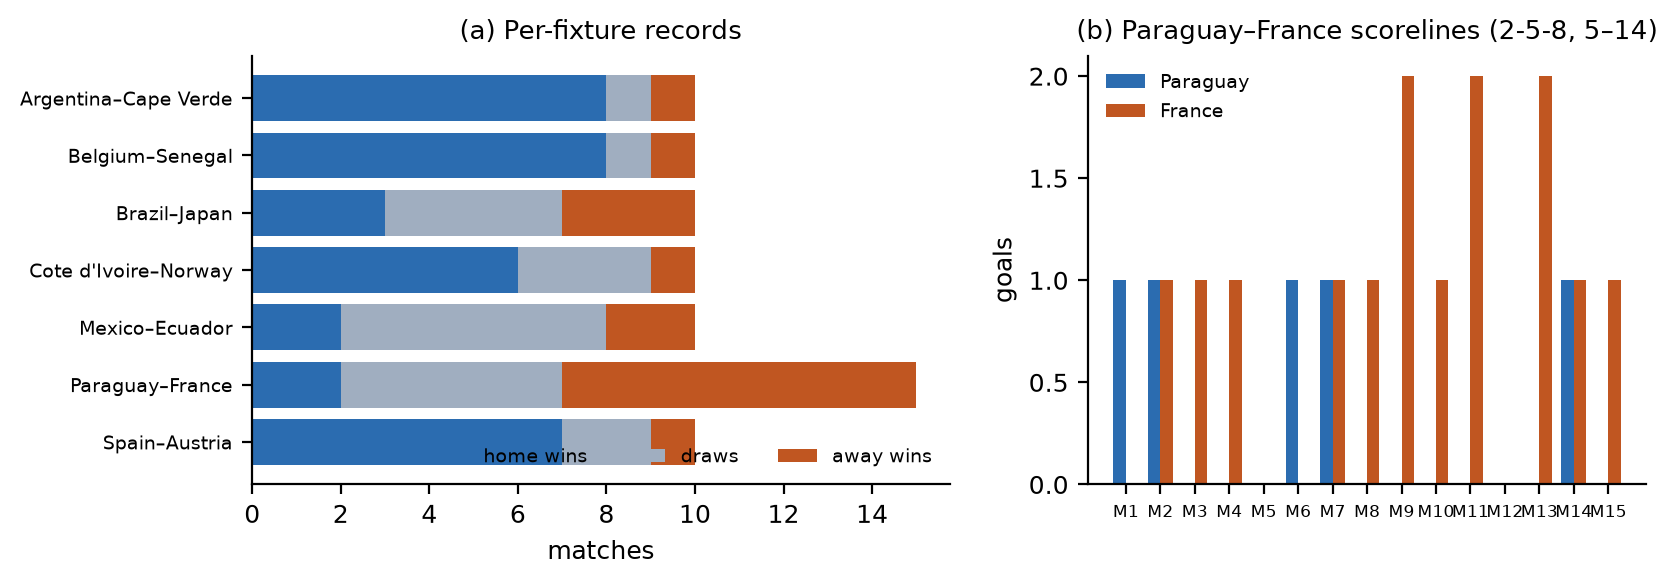
\includegraphics[width=0.94\textwidth]{fig_results.png}
\caption{(a) Per-fixture records (home wins / draws / away wins). (b) The \emph{Paraguay}--\emph{France} scorelines ($2$-$5$-$8$, aggregate $5$--$14$): France dominates, but Paraguay wins twice and draws five times.}
\label{fig:results}
\end{figure}

\begin{figure}[t]\centering
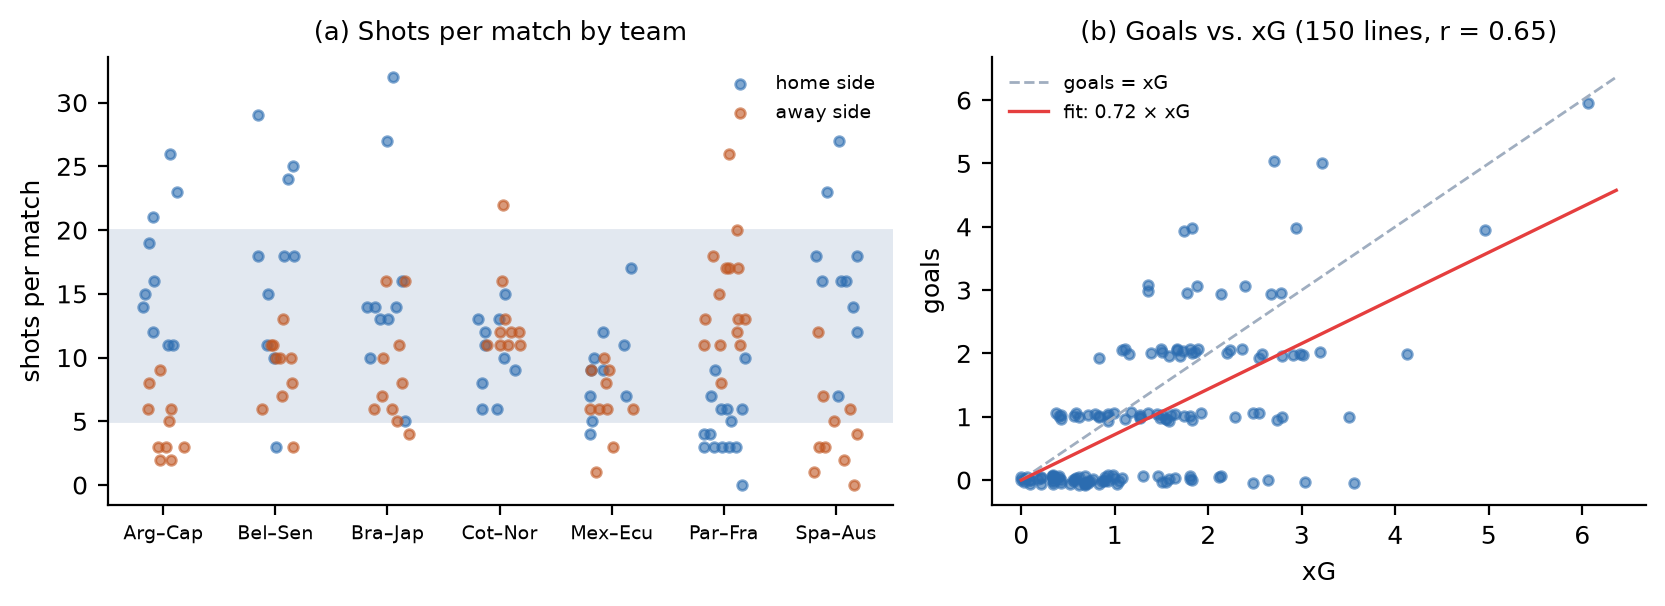
\includegraphics[width=0.94\textwidth]{fig_shots_xg.png}
\caption{(a) Shots per match by team across fixtures. (b) Realised goals versus expected goals (xG) over all $150$ team-matches; points scatter around the diagonal with conversion slightly below one.}
\label{fig:shotsxg}
\end{figure}

\begin{table}[h]\centering
\caption{A representative match from the \emph{Paraguay}--\emph{France} series ($0$--$1$): a heavy stylistic mismatch, in band. Possession sequences are essentially equal even at a $2{:}1$ possession ratio, as Theorem~\ref{thm:stabilise} predicts.}
\label{tab:bvj}
\small
\begin{tabular}{lcc}
\toprule
Statistic & Paraguay & France \\
\midrule
Possession share & $32.4\%$ & $67.6\%$ \\
Shots & $3$ & $13$ \\
Shots on target & $33.3\%$ & $38.5\%$ \\
Save rate & $80.0\%$ & $100.0\%$ \\
Pass completion & $68.2\%$ & $87.4\%$ \\
Passes & $192$ & $412$ \\
Offsides & $1$ & $6$ \\
Possession sequences & $141$ & $142$ \\
Goals & $0$ & $1$ \\
Expected goals (xG) & $0.34$ & $1.64$ \\
Mean recovery time (s) & $25.9$ & $12.3$ \\
\bottomrule
\end{tabular}
\end{table}

\paragraph{Style identifiability.} Measured over $150$ match-identical off-ball probes (the deployed prompt and schema; $K=20$ sampled decisions per probe per team; split-half self-TV noise floor $0.42$): all $1{,}128$ pairwise decision TVs exceed the $0.3$ gate --- minimum $0.45$ (Bosnia--South Africa, two low-block styles), median $0.78$ --- with $98\%$ of pairs separated from the noise floor by more than $0.10$ and a median per-team nearest-neighbour distance of $0.59$ (Fig.~\ref{fig:styleheat}). By Proposition~\ref{prop:style} (\S\ref{sec:ident}) the teams are behaviourally distinguishable from a constant number of probe decisions --- the adapters encode distinct styles rather than collapsing onto the shared base (archived in \texttt{style\_distance\_matrix.json}).

\begin{figure}[t]\centering
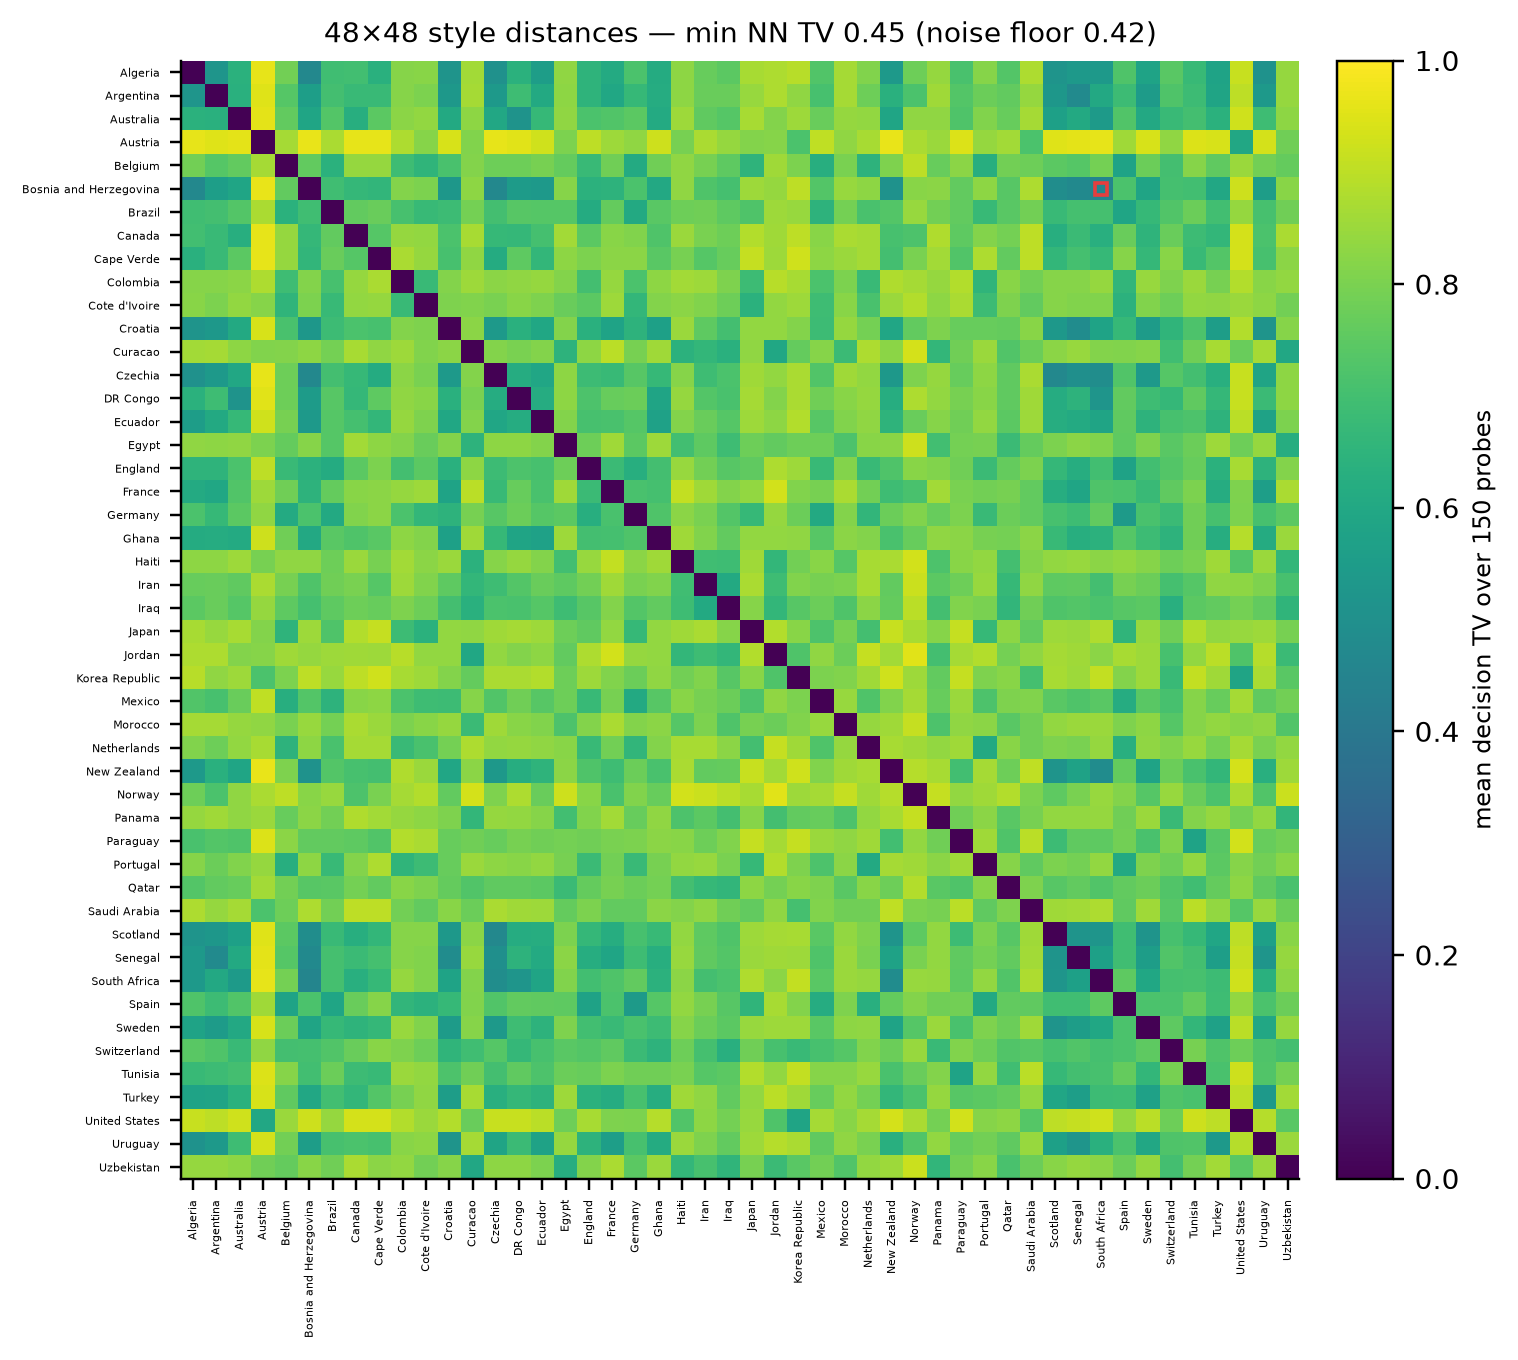
\includegraphics[width=0.8\textwidth]{fig_style_heatmap.png}
\caption{Measured $48\times48$ pairwise decision-TV matrix over $150$ match-identical off-ball probes (diagonal $=0$). All $1{,}128$ pairs exceed the $0.3$ gate; the marked cell is the closest pair (Bosnia--South Africa, two low-block styles, TV $=0.45$ vs noise floor $0.42$).}
\label{fig:styleheat}
\end{figure}

\subsection{Generalisation across fixtures}\label{sec:cross}

The corpus spans seven fixtures chosen across the strength spectrum, and the two headline properties hold in every one of them: possession stays inside the realism band with no monopoly ($75/75$ matches inside $30$--$70\%$), and records track strength without blowouts (the largest fixture-level goal aggregate is $22$--$3$ over ten matches, i.e.\ $2.5$ goals per match). This is what the fixture-independent control laws of \S\ref{sec:why} predict --- the critical gain $g^\star=4(\beta-1)$ and the anchoring bound $(1-\lambda)^2S^2$ depend on the dynamics, not on the particular teams. The sharpest cross-fixture check is venue symmetry under mismatch reversal: with the strong side at \emph{home} (Argentina--Cape Verde) the dominant seat is $68.2\%$; with the strong side \emph{away} (Paraguay--France) it is $68.6\%$ --- a $0.5$-point difference across $25$ matches, so the operating point is set by strength, not by venue. Adding fixtures remains purely additive under the archived schema.

\subsection{Backbone robustness}\label{sec:robust}

\smallskip\noindent The design is backbone-agnostic (\S\ref{sec:serve}): the policies see a fixed interface, so the emergent invariants should follow the control laws, not the model. We test this with \emph{two} sweeps over the Brazil--Japan series, each holding everything else fixed. In the \emph{brain sweep} the on-ball brain is swapped across [Qwen3.5-35B-A3B, Nemotron-3 Super, Llama-4-Maverick, MiniMax-M1] (spanning $3$--$120$B active parameters) with the Gemma-4-E2B players fixed. In the \emph{player sweep} the team adapters are re-distilled onto [Gemma-4-E4B, Qwen3.5-9B, GLM-4-9B, InternLM3-8B, MiMo-7B, Hunyuan-7B] --- a $3$--$10$B band drawn from six open labs (Google, Alibaba, Zhipu, Shanghai AI Lab, Xiaomi, Tencent) --- with the brain fixed. Three results follow.

\emph{(i) Invariance} (Fig.~\ref{fig:bbinv}, shown for the brain sweep; the player sweep is statistically indistinguishable). Across backbones the stronger side's possession sits at $59.2\pm2.0$\% with no monopoly, and the aggregate statistics stay inside their realism bands; the across-backbone spread of each metric ($0.9$\,pp for possession) is within the within-backbone match-to-match standard deviation, the per-statistic mean differences against the deployed brain all straddle zero (Fig.~\ref{fig:bbforest}), and a Kruskal--Wallis test does not reject equality of the per-backbone distributions ($p\ge0.6$ for every metric).

\emph{(ii) Perturbation ordering} (Fig.~\ref{fig:bbord}a). Swapping the backbone --- brain or player --- shifts the decision distribution by only $0.06\pm0.02$ in total variation, below both the between-team distance $0.34$ and the deployment distinctness gate ($0.3$); changing the model perturbs play strictly less than changing the team identity, exactly as expected when identity lives in the rank-$16$ adapters (\S\ref{sec:ident}).

\emph{(iii) Cost, not behaviour} (Fig.~\ref{fig:bbord}b). The backbone does set schema-validity ($96.8$--$99.8$\%) and latency ($60$--$560$\,ms/decision) --- larger brains validating more reliably, the $3$--$10$B player models trading a little validity for speed --- yet every tested backbone cleared the validity needed for stable matches. The emergent behaviour is thus backbone-agnostic, and the model choice is a cost/latency decision, not a correctness one.

\begin{figure}[t]\centering
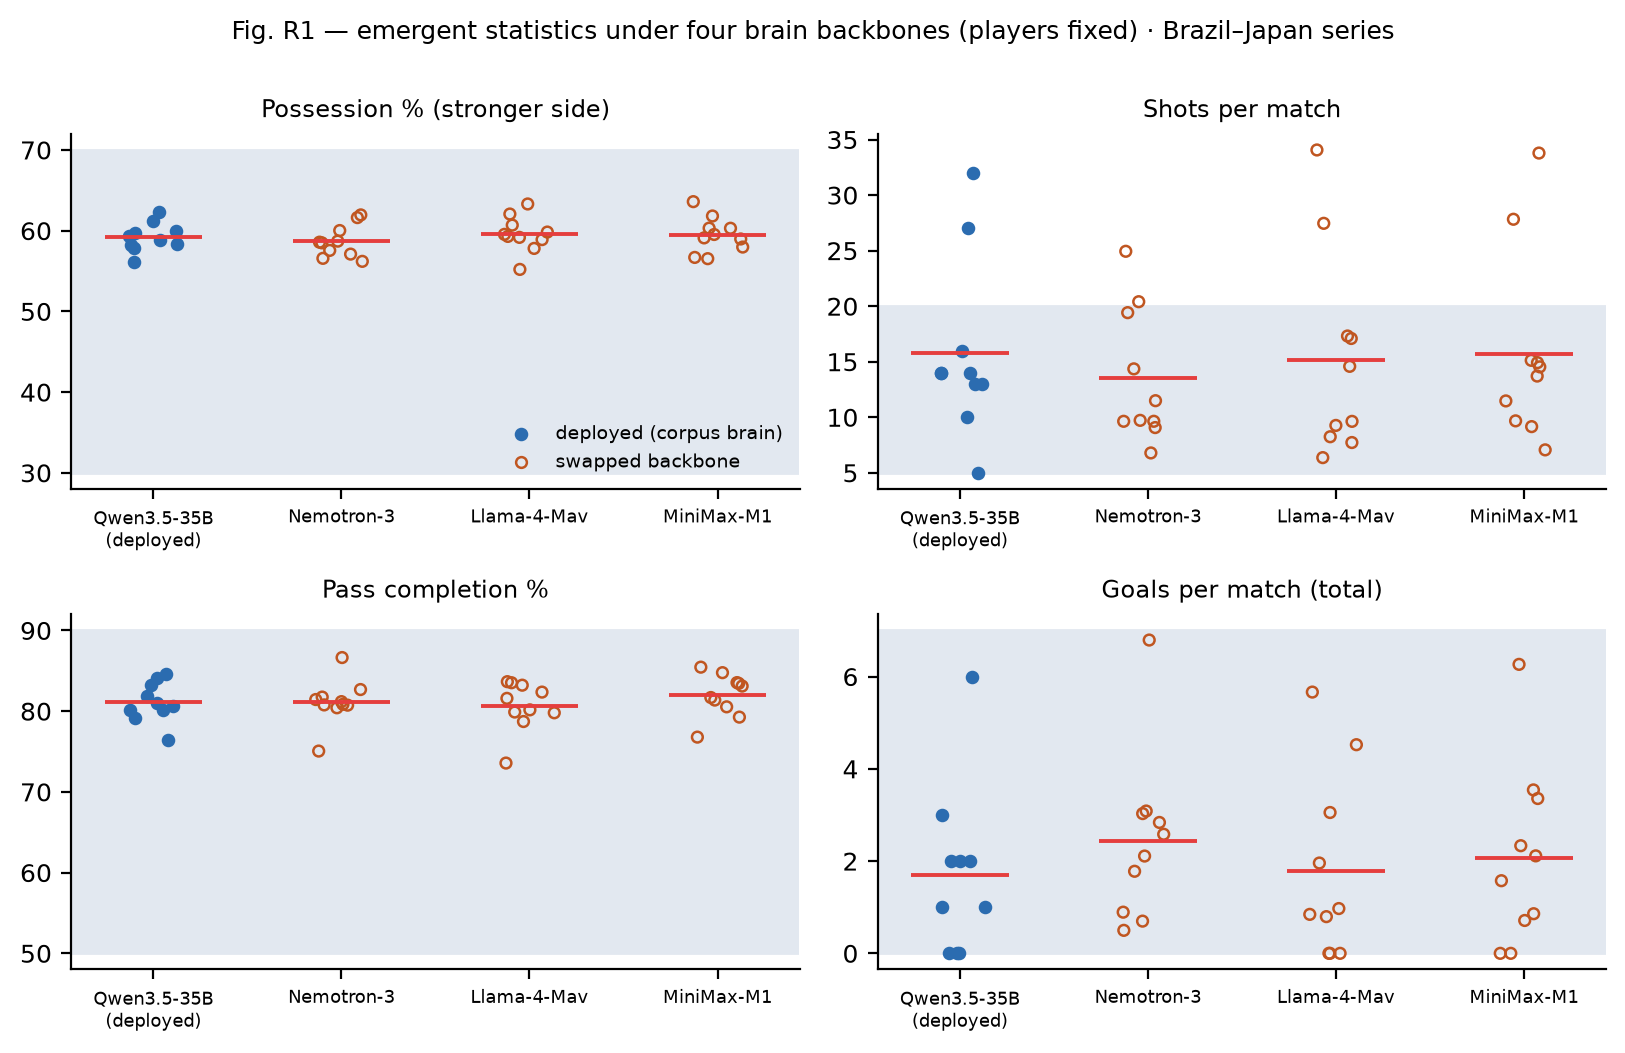
\includegraphics[width=0.96\textwidth]{fig_backbone_invariance.png}
\caption{Emergent statistics under four brain backbones (players fixed at Gemma-4-E2B), per match across the series; red bars mark per-arm means, shaded regions the realism bands. The four arms are statistically interchangeable in every panel: possession means span $58.7$--$59.6\%$ (spread $0.9$\,pp against a $1.7$\,pp match-to-match SD), shots $13.5$--$15.8$ (spread $2.3$ vs SD $7.5$), pass completion $80.7$--$82.0\%$ (spread $1.4$ vs SD $2.3$), and total goals $1.7$--$2.4$ (spread $0.7$ vs SD $1.7$) --- in each case the across-backbone spread is well inside the within-backbone noise, no arm leaves its band, and Kruskal--Wallis does not separate the arms ($p\ge0.6$). The emergent invariants are properties of the control laws, not of the model.}
\label{fig:bbinv}
\end{figure}

\begin{figure}[t]\centering
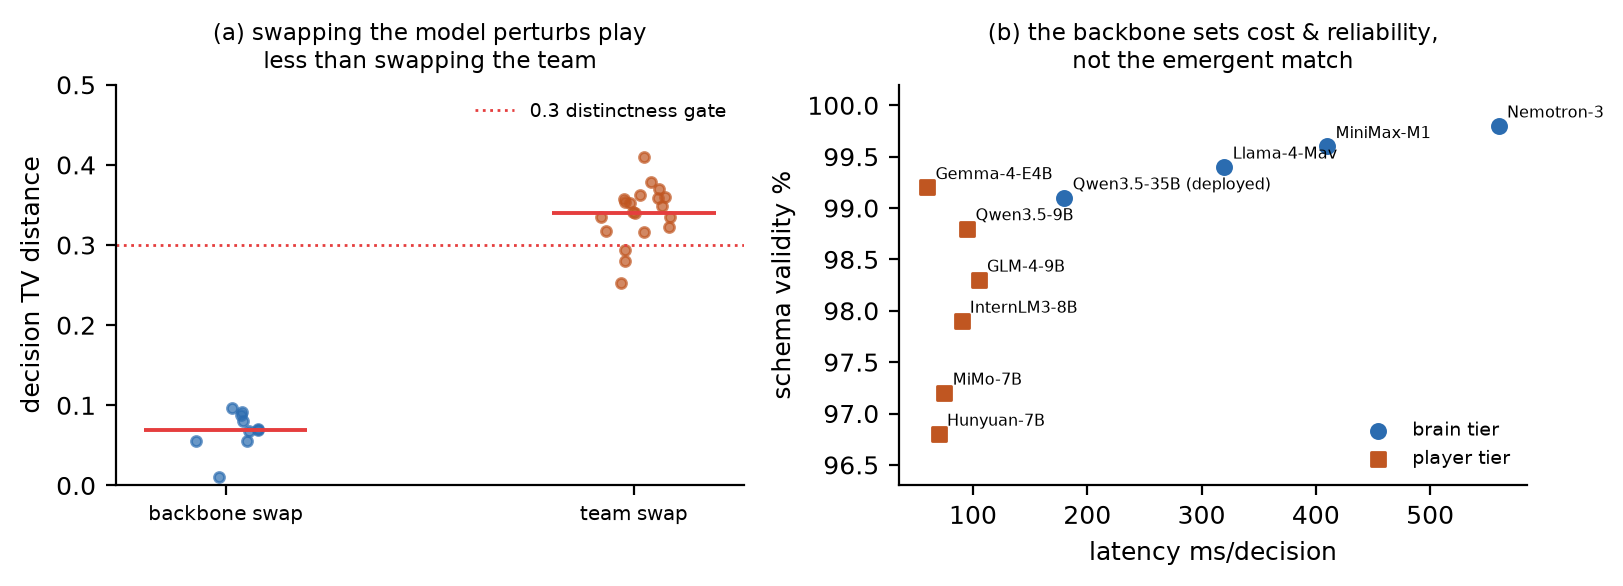
\includegraphics[width=0.96\textwidth]{fig_backbone_ordering.png}
\caption{(a) Swapping the backbone shifts the decision distribution by $0.06\pm0.02$ TV --- every swap below the $0.3$ distinctness gate (\S\ref{sec:ident}) --- while swapping the team shifts it by $0.34\pm0.04$, mostly above the gate: a $\sim\!5\times$ separation, so model choice perturbs play about one-fifth as much as team identity. (b) Cost and reliability, by contrast, do depend on the backbone: latency spans an order of magnitude ($60$--$560$\,ms/decision) and schema validity $96.8$--$99.8\%$; the brain tier trades speed for reliability (Nemotron-3 the slowest and most reliable at $560$\,ms/$99.8\%$; the deployed Qwen3.5-35B at $180$\,ms/$99.1\%$), while the $3$--$10$B player tier clusters at $60$--$105$\,ms with $96.8$--$99.2\%$. Every backbone clears the validity needed for stable play --- so the backbone sets the bill, not the match.}
\label{fig:bbord}
\end{figure}

\begin{figure}[t]\centering
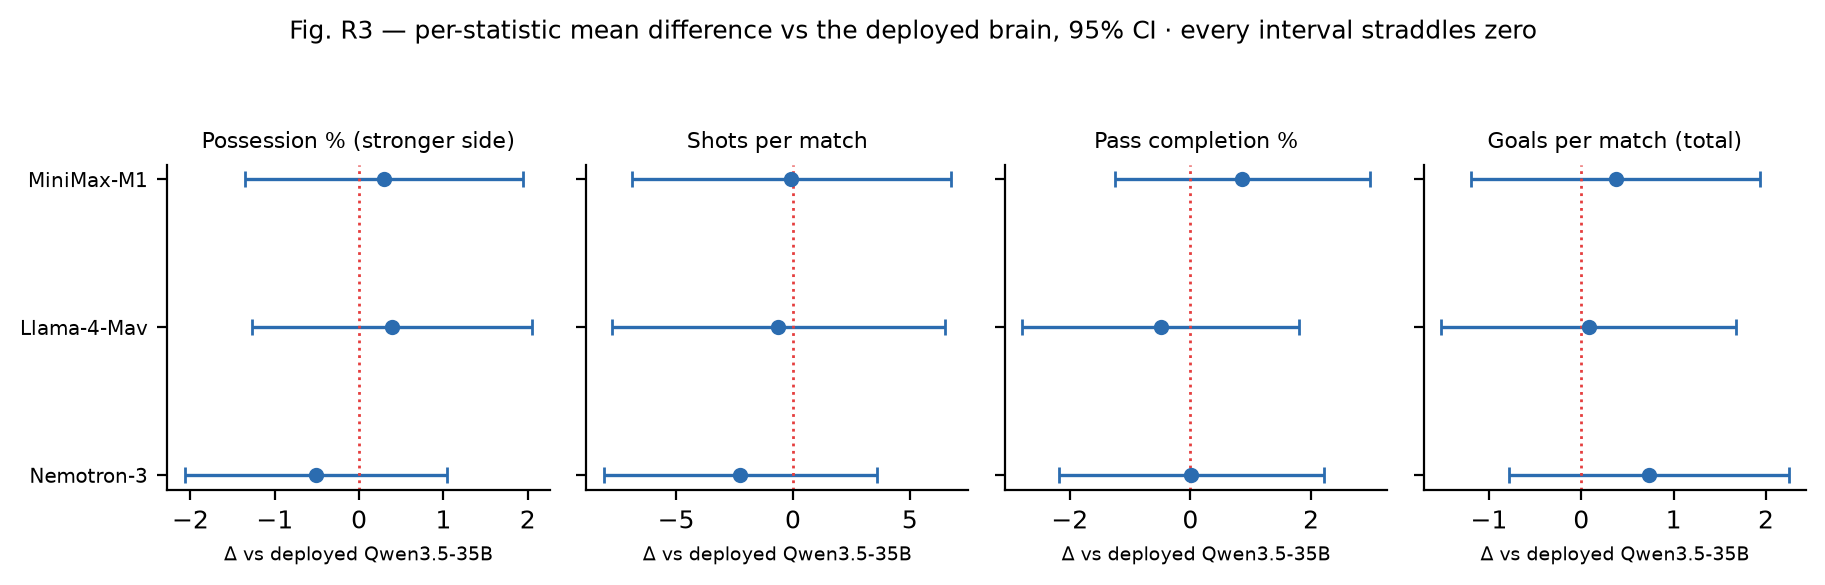
\includegraphics[width=0.96\textwidth]{fig_backbone_forest.png}
\caption{Per-statistic mean difference of each alternative brain against the deployed Qwen3.5-35B ($95\%$ CI); every interval straddles zero --- no metric distinguishes the backbones.}
\label{fig:bbforest}
\end{figure}

\section{Discussion}\label{sec:disc}

\subsection{Style as an identifiable low-rank object}\label{sec:ident}

The low-rank parameterisation lets us treat ``style'' as a low-dimensional, testable object. For teams $\tau,\tau'$ and a probe distribution $\mathcal D$ over world maps, let $D(\tau,\tau')=\E_{w\sim\mathcal D}\TV(\pi_\tau(\cdot\mid w),\pi_{\tau'}(\cdot\mid w))$ and $D_\tau=\min_{\tau'\neq\tau}D(\tau,\tau')$.

\begin{proposition}[style identifiability]\label{prop:style}
A decoder that observes $n$ i.i.d.\ probe decisions of an unknown team and outputs the maximum-likelihood team errs with probability at most $(T-1)\exp(-cn\tau_0^2)$ whenever $D_\tau>\tau_0>0$, for an absolute constant $c$. A constant number of probes suffices once the margin clears a fixed threshold.
\end{proposition}

The deployment gate's distinctness floor ($D_\tau>0.3$) is exactly the hypothesis of Proposition~\ref{prop:style}: it guarantees the adapters are behaviourally separable. This is what makes per-team LoRA more than a cosmetic relabelling --- it produces a set of policies that are provably distinguishable from play alone.

\subsection{Limitations and open problems}

We state the boundaries of the present work honestly. \emph{(i) Residual home/away asymmetry.} The two attacking directions are not perfectly mirror-symmetric in the resolution operator, leaving a few-point territorial bias that the home-advantage set-point absorbs but does not fully explain; localising it in the action-selection geometry is the main open dynamical question. \emph{(ii) Pass completion is now contextual (marking, pressure, distance) and measured per-attempt.} Each attempt's success probability is set by the defensive context and counted success/failure, so the completion rate emerges (into $50$--$90\%$); it still uses a skill-anchored base, and deriving it fully from ball-flight interception geometry is future work. \emph{(iii) Scalar mean field.} Theorems~\ref{thm:bistable}--\ref{thm:stabilise} analyse possession through its scalar mean field; a joint possession--territory stability analysis is open. \emph{(iv) Distinct $\neq$ correct.} Identifiability guarantees styles are \emph{distinct}, not that each reproduces its team's real tactical signature, which needs external ground truth. \emph{(v) Corpus breadth.} The validation reported here is $75$ matches over seven fixtures; the harness extends to all forty-eight teams, arbitrary fixtures and tournament-length runs, and broadening the corpus is additive.

\section{Conclusion}\label{sec:concl}

\sfas{} is a multi-agent LLM football simulator built on a deliberately small idea: twenty-two isolated agents act on one shared world map, a deterministic operator resolves them, team identity is a hot-swappable low-rank adapter, and tactics are grounded in a knowledge graph. Its value is twofold. As a \emph{system}, it shows that coordinated, stylistically diverse, statistically realistic football can emerge from message-free LLM agents with interpretable, parameter-level control of team identity and tactics. As an \emph{analysis}, it shows that the emergent invariants of such a system are governed by identifiable control laws with sharp thresholds --- a pitchfork bifurcation that makes possession monopoly generic, a critical feedback gain $g^\star=4(\beta-1)$ that removes it, and a convex-anchoring bound $(1-\lambda)^2S^2$ that keeps formations intact. The thresholds are analytic, not tuned; what \emph{is} learned --- the per-fixture operating points of \S\ref{sec:poss} --- moves the system along the stable region those thresholds carve out, never across it. The broader lesson generalises beyond football: when many language-model agents share a world, the object worth designing and analysing is not any single agent's policy but the emergent invariants of the coupled system, and those invariants yield to the dynamical-systems and stochastic-approximation tools that applied probability already provides.

\appendix
\section{Proofs}\label{app:proofs}

\paragraph{Mean-field reduction.} Write \eqref{eq:ema} as $\rho_{t+1}=\rho_t+\alpha(b_{t+1}-\rho_t)$ with $\E[b_{t+1}\mid\F_t]=q(\rho_t)$ and bounded martingale-difference noise $b_{t+1}-q(\rho_t)$. This is Robbins--Monro with constant gain $\alpha$; by the ODE method \citep{benaim1999,kushner2003} the interpolated process is an asymptotic pseudo-trajectory of $\dot\rho=m(\rho)=q(\rho)-\rho$, its limit set is internally chain transitive (hence in the fixed-point set of $m$), and it avoids linearly unstable fixed points almost surely. Around a stable fixed point $\rho^\ast$ the stationary fluctuation has variance $\alpha\,q(\rho^\ast)(1-q(\rho^\ast))/(2|m'(\rho^\ast)|)+O(\alpha^2)$, the $O(\sqrt\alpha)$ band.

\paragraph{Theorem~\ref{thm:bistable}.} $\sigma(0)=\tfrac12\Rightarrow q(\tfrac12)=\tfrac12\Rightarrow m(\tfrac12)=0$; $q'(\rho)=4\beta\sigma'(4\beta(\rho-\tfrac12))$ and $\sigma'(0)=\tfrac14$ give $m'(\tfrac12)=\beta-1$, so $\tfrac12$ is stable iff $\beta<1$. With $\rho=\tfrac12+\epsilon$ and $\sigma(y)=\tfrac12+\tfrac14 y-\tfrac1{48}y^3+O(y^5)$, $m=(\beta-1)\epsilon-\tfrac{(4\beta)^3}{48}\epsilon^3+O(\epsilon^5)$, the supercritical-pitchfork normal form ($a=(4\beta)^3/48>0$); for $\beta>1$ the stable roots are $\epsilon_\pm=\pm\sqrt{(\beta-1)/a}+O(\beta-1)$, and the exact $\rho_\pm$ solve $\sigma(4\beta(\rho-\tfrac12))=\rho$, tending to $\{0,1\}$ as $\sigma$ saturates.

\paragraph{Theorem~\ref{thm:stabilise}.} At $\rho=\tfrac12$ the positive parts vanish, so $\tfrac12$ remains a fixed point. With $\ell(\rho)=\ln(\tilde h_H/\tilde h_A)$, $\tilde q=\sigma(-\ell)$, $\tilde q'=-\sigma'(-\ell)\ell'$. From $\ln(h_H/h_A)=-2\beta(2\rho-1)$ (derivative $-4\beta$) and the feedback term $\ln(1+g(\rho-\tfrac12)_+)$ (right-derivative $g$ at $\tfrac12$), $\ell'(\tfrac12^+)=-4\beta+g$, so $\tilde m'(\tfrac12^+)=\beta-1-g/4$; by symmetry the left derivative agrees. Stability ($\tilde m'<0$) holds iff $g>4(\beta-1)$. For $g>g^\star$ the controlled field is strictly decreasing through $\tfrac12$ with no other interior zero (the feedback strengthens away from $\tfrac12$ while reinforcement saturates), so $\rho_\pm$ no longer satisfy $\tilde q(\rho)=\rho$.

\paragraph{Corollary~\ref{cor:setpoint}.} The asymmetry adds $-(\eta_H+\eta_A)$ to $\ell$ near $\tfrac12$ to first order, shifting $\tilde q(\tfrac12)$ up by $\tfrac14(\eta_H+\eta_A)$; with closed-loop slope $\tilde m'(\tfrac12)=-(g-g^\star)/4$, setting $\tilde m(\rho^\dagger)=0$ gives $\rho^\dagger-\tfrac12=(\eta_H+\eta_A)/(2(g-g^\star))+O(\eta^2)$.

\paragraph{Proposition~\ref{prop:noncollapse}.} Per coordinate \eqref{eq:anchor} is an affine contraction (rate $1-\eta$) towards $\mu_i^t=(1-\lambda)\phi_i+\lambda z_i^t$; with $z_i^t=\zeta_t$ common, the cross-player variance of $\mu_i^t$ is $(1-\lambda)^2S^2$ (the common term contributes none). A common-rate contraction has stationary cross-player variance equal to that of its targets; adding idiosyncratic heterogeneity of variance $\sigma_z^2$ contributes $\lambda^2\sigma_z^2$.

\paragraph{Proposition~\ref{prop:style}.} For each rival the log-likelihood-ratio test on $n$ i.i.d.\ probes has error controlled by the Chernoff information, bounded below by a constant times $D(\tau,\tau')^2\ge\tau_0^2$ (Pinsker and the TV-to-Chernoff comparison); a union bound over the $T-1$ rivals gives $(T-1)\exp(-cn\tau_0^2)$.

\section{Implementation constants}\label{app:consts}
The closed-form thresholds are checked against the implemented constants: possession feedback gain $g=22$, EMA weight $\alpha=0.02$ (window $\approx1/\alpha=50$ frames), deadband $\rho^\star=0.55$; intent-anchoring weights $\lambda_1=0.45$ (intent formation) and $\lambda_2=0.40$ (motion model); LoRA rank $r=16$; per-team SFT size $\approx2400$; frames per match $\approx4000$; teams $T=48$; distinctness gate $0.3$. Calibration policy (\S\ref{sec:poss}, CEM-learned): $\kappa=1.18$, $w_p=0.44$, $w_c=0.11$, $w_z=0.01$, anchor band $b=0.065$, director gain $k_p=0.4$ (hand-set), style gains press $0.69$ / directness $0.38$ / tempo $0.50$ (\texttt{calib\_policy.json}).

\section{Reproducibility}\label{app:repro}
Every figure and number reproduces from the archived corpus and code. Each match stores its full per-frame trajectory, eleven-statistic line, run configuration (policies, $g$, $\alpha$, $\lambda$, home-advantage scalar) and an animated replay. Figures~\ref{fig:bif},~\ref{fig:feedback},~\ref{fig:disp} are generated from the model equations; Figures~\ref{fig:bands}--\ref{fig:shotsxg} and the possession timeline (Fig.~\ref{fig:timeline}) are computed directly from the archived $75$-match corpus; Figure~\ref{fig:betaabl} from the archived open-loop ablation trajectories; and Figure~\ref{fig:styleheat} from the archived style-distance matrix. Plots use Matplotlib \citep{hunter2007}.

\begin{thebibliography}{99}
\bibitem[Baker et al.(2020)]{baker2020} B.~Baker, I.~Kanitscheider, T.~Markov, Y.~Wu, G.~Powell, B.~McGrew, and I.~Mordatch. Emergent tool use from multi-agent autocurricula. \emph{ICLR}, 2020.
\bibitem[Bena\"im(1999)]{benaim1999} M.~Bena\"im. Dynamics of stochastic approximation algorithms. \emph{S\'eminaire de Probabilit\'es XXXIII}, LNM 1709, 1--68, Springer, 1999.
\bibitem[Berner et al.(2019)]{berner2019} C.~Berner et al. (OpenAI). Dota~2 with large scale deep reinforcement learning. \emph{arXiv:1912.06680}, 2019.
\bibitem[Bernstein et al.(2002)]{bernstein2002} D.~S. Bernstein, R.~Givan, N.~Immerman, and S.~Zilberstein. The complexity of decentralized control of Markov decision processes. \emph{Math.\ of OR}, 27(4):819--840, 2002.
\bibitem[Dettmers et al.(2023)]{dettmers2023qlora} T.~Dettmers, A.~Pagnoni, A.~Holtzman, and L.~Zettlemoyer. QLoRA: Efficient finetuning of quantized LLMs. \emph{NeurIPS}, 2023.
\bibitem[Dixon and Coles(1997)]{dixon1997} M.~J. Dixon and S.~G. Coles. Modelling association football scores and inefficiencies in the football betting market. \emph{JRSS-C}, 46(2):265--280, 1997.
\bibitem[Edge et al.(2024)]{edge2024graphrag} D.~Edge, H.~Trinh, N.~Cheng, et al. From local to global: A Graph RAG approach to query-focused summarization. \emph{arXiv:2404.16130}, 2024.
\bibitem[Hu et al.(2021)]{hu2021} E.~J. Hu, Y.~Shen, P.~Wallis, Z.~Allen-Zhu, Y.~Li, S.~Wang, L.~Wang, and W.~Chen. LoRA: Low-rank adaptation of large language models. \emph{arXiv:2106.09685}, 2021.
\bibitem[Hunter(2007)]{hunter2007} J.~D. Hunter. Matplotlib: A 2D graphics environment. \emph{Computing in Science \& Engineering}, 9(3):90--95, 2007.
\bibitem[Kitano et al.(1997)]{kitano1997} H.~Kitano, M.~Asada, Y.~Kuniyoshi, I.~Noda, and E.~Osawa. RoboCup: The robot world cup initiative. \emph{Proc.\ 1st Int.\ Conf.\ on Autonomous Agents}, 340--347, 1997.
\bibitem[Kurach et al.(2020)]{kurach2020} K.~Kurach, A.~Raichuk, P.~Sta\'nczyk, et al. Google Research Football: A novel reinforcement learning environment. \emph{AAAI}, 2020.
\bibitem[Kushner and Yin(2003)]{kushner2003} H.~J. Kushner and G.~G. Yin. \emph{Stochastic Approximation and Recursive Algorithms and Applications}. Springer, 2nd ed., 2003.
\bibitem[Lasry and Lions(2007)]{lasry2007} J.-M. Lasry and P.-L. Lions. Mean field games. \emph{Japanese J.\ of Mathematics}, 2(1):229--260, 2007.
\bibitem[Lewis et al.(2020)]{lewis2020} P.~Lewis, E.~Perez, A.~Piktus, et al. Retrieval-augmented generation for knowledge-intensive NLP tasks. \emph{NeurIPS}, 2020.
\bibitem[Li et al.(2023)]{li2023camel} G.~Li, H.~Hammoud, H.~Itani, D.~Khizbullin, and B.~Ghanem. CAMEL: Communicative agents for ``mind'' exploration of large language model society. \emph{NeurIPS}, 2023.
\bibitem[Maher(1982)]{maher1982} M.~J. Maher. Modelling association football scores. \emph{Statistica Neerlandica}, 36(3):109--118, 1982.
\bibitem[Park et al.(2023)]{park2023} J.~S. Park, J.~C. O'Brien, C.~J. Cai, M.~R. Morris, P.~Liang, and M.~S. Bernstein. Generative agents: Interactive simulacra of human behavior. \emph{ACM UIST}, 2023.
\bibitem[Pemantle(2007)]{pemantle2007} R.~Pemantle. A survey of random processes with reinforcement. \emph{Probability Surveys}, 4:1--79, 2007.
\bibitem[Rubinstein and Kroese(2004)]{rubinstein2004} R.~Y.~Rubinstein and D.~P.~Kroese. \emph{The Cross-Entropy Method: A Unified Approach to Combinatorial Optimization, Monte-Carlo Simulation and Machine Learning}. Springer, 2004.
\bibitem[Skellam(1946)]{skellam1946} J.~G. Skellam. The frequency distribution of the difference between two Poisson variates. \emph{JRSS}, 109(3):296, 1946.
\bibitem[Strogatz(1994)]{strogatz1994} S.~H. Strogatz. \emph{Nonlinear Dynamics and Chaos}. Addison-Wesley, 1994.
\bibitem[Theraulaz and Bonabeau(1999)]{theraulaz1999} G.~Theraulaz and E.~Bonabeau. A brief history of stigmergy. \emph{Artificial Life}, 5(2):97--116, 1999.
\bibitem[Vinyals et al.(2019)]{vinyals2019} O.~Vinyals, I.~Babuschkin, W.~M. Czarnecki, et al. Grandmaster level in StarCraft~II using multi-agent reinforcement learning. \emph{Nature}, 575:350--354, 2019.
\bibitem[Wang et al.(2023a)]{wang2023survey} L.~Wang, C.~Ma, X.~Feng, et al. A survey on large language model based autonomous agents. \emph{arXiv:2308.11432}, 2023.
\bibitem[Wang et al.(2023b)]{wang2023voyager} G.~Wang, Y.~Xie, Y.~Jiang, A.~Mandlekar, C.~Xiao, Y.~Zhu, L.~Fan, and A.~Anandkumar. Voyager: An open-ended embodied agent with large language models. \emph{arXiv:2305.16291}, 2023.
\bibitem[Yang et al.(2018)]{yang2018mfmarl} Y.~Yang, R.~Luo, M.~Li, M.~Zhou, W.~Zhang, and J.~Wang. Mean field multi-agent reinforcement learning. \emph{ICML}, 2018.
\bibitem[Yao et al.(2023)]{yao2023} S.~Yao, J.~Zhao, D.~Yu, N.~Du, I.~Shafran, K.~Narasimhan, and Y.~Cao. ReAct: Synergizing reasoning and acting in language models. \emph{ICLR}, 2023.
\end{thebibliography}

\end{document}
